% This must be in the first 5 lines to tell arXiv to use pdfLaTeX, which is strongly recommended.
\pdfoutput=1
% In particular, the hyperref package requires pdfLaTeX in order to break URLs across lines.

\documentclass[11pt]{article}

% Change "review" to "final" to generate the final (sometimes called camera-ready) version.
% Change to "preprint" to generate a non-anonymous version with page numbers.
\usepackage[preprint]{acl}

% Standard package includes
% \usepackage{times}
\usepackage{newtxmath}
\usepackage{newtxtext}

\usepackage{fix-cm}
\usepackage{latexsym}


% For proper rendering and hyphenation of words containing Latin characters (including in bib files)
\usepackage[T1]{fontenc}
% For Vietnamese characters
% \usepackage[T5]{fontenc}
% See https://www.latex-project.org/help/documentation/encguide.pdf for other character sets

% This assumes your files are encoded as UTF8
\usepackage[utf8]{inputenc}

% This is not strictly necessary, and may be commented out,
% but it will improve the layout of the manuscript,
% and will typically save some space.
\usepackage{microtype}

% This is also not strictly necessary, and may be commented out.
% However, it will improve the aesthetics of text in
% the typewriter font.
\usepackage{inconsolata}

%Including images in your LaTeX document requires adding
%additional package(s)
\usepackage{graphicx}

% If the title and author information does not fit in the area allocated, uncomment the following
%
%\setlength\titlebox{<dim>}
%
% and set <dim> to something 5cm or larger.

%\usepackage{hyperref}
\usepackage{booktabs}
\usepackage{standalone}
\usepackage{tikz}
\usepackage{pgfplots}
\usepackage{siunitx}
\sisetup{table-format=2.1,detect-all = true}
\usepackage{multirow, xcolor, colortbl}
\usepackage{soul}
\usepackage{hhline}
\usepackage{etoolbox}
\usepackage[capitalize]{cleveref}
\usepackage{caption}
\usepackage{subcaption}
\usepackage{relsize}
\usepackage{threeparttable}
\usepackage{tabularx}

\pgfplotsset{compat=newest}
\usepgfplotslibrary{groupplots}

\robustify\bfseries
\usetikzlibrary{positioning, patterns, fit}

\usepackage{xspace}
\newcommand\ours{SD-RA-IT\xspace}
\newcommand\baseline{RA-IT\xspace}
\newcommand\llamainstruct{Llama-3-Instruct\xspace}
\newcommand\llamasmall{Llama-3-8B-Instruct\xspace}
\newcommand\llamabig{Llama-3-70B-Instruct\xspace}
\newcommand\llamahuge{Llama-3.1-405B-Instruct\xspace}
\hyphenation{O-pen-As-sis-tant}

\newcommand{\barlas}[1]{\textcolor{red}{Barlas: #1}}
\newcommand{\matt}[1]{\textcolor{blue}{Matt: #1}}
\newcommand{\xilun}[1]{\textcolor{purple}{Xilun: #1}}

\title{Post-training an LLM for RAG? Train on Self-Generated Demonstrations}

\author{
  Matthew Finlayson\footnotemark[1]
  \quad Ilia Kulikov\footnotemark[2]
  \quad Daniel M. Bikel\footnotemark[2] \\
  \bf \quad Barlas Oguz\footnotemark[2]
  \quad Xilun Chen\footnotemark[2] 
  \quad Aasish Pappu\footnotemark[2] \\
  \footnotemark[1]University of Southern California
  \quad \footnotemark[2]Meta, Inc.
  \\
  \texttt{mfinlays@usc.edu}\quad\texttt{aasish@meta.com}
}

\begin{document}
\maketitle

\begin{abstract}
  \begin{abstract}  
Test time scaling is currently one of the most active research areas that shows promise after training time scaling has reached its limits.
Deep-thinking (DT) models are a class of recurrent models that can perform easy-to-hard generalization by assigning more compute to harder test samples.
However, due to their inability to determine the complexity of a test sample, DT models have to use a large amount of computation for both easy and hard test samples.
Excessive test time computation is wasteful and can cause the ``overthinking'' problem where more test time computation leads to worse results.
In this paper, we introduce a test time training method for determining the optimal amount of computation needed for each sample during test time.
We also propose Conv-LiGRU, a novel recurrent architecture for efficient and robust visual reasoning. 
Extensive experiments demonstrate that Conv-LiGRU is more stable than DT, effectively mitigates the ``overthinking'' phenomenon, and achieves superior accuracy.
\end{abstract}  
\end{abstract}

\begin{figure*}
  \centering
  \small
  \newcommand{\boformat}[1]{$\mathbf{#1}$}
\newcommand{\blformat}[1]{\textcolor{blue}{$\mathbf{#1}$}}

\def\arraystretch{1.1}
\setlength{\tabcolsep}{0.5em} %

\begin{table}[t!] \centering
    \caption{Comparison of TD3 with existing dataset distillation techniques and heuristic sampling based methods.
    }
    \vspace{-8pt}
    \label{tab:baselines}
    \begin{center}
    \resizebox{0.48\textwidth}{!}{
    \begin{tabular}{cc|cc|cc|c}
        \toprule
        \multirow{2.8}{*}{Dataset} & \multirow{2.8}{*}{Metric} & \multicolumn{2}{c|}{Sampling} & \multicolumn{2}{c|}{Distillation} & \multirow{2.8}{*}{Full-Data} \\[3pt]
        
        \cmidrule{3-6}
        & & \multicolumn{1}{c}{Random.} & \multicolumn{1}{c|}{Longest.} & \multicolumn{1}{c}{Farzi} & \multicolumn{1}{c|}{\sampler} \\[2pt]
        
        \midrule
        \multirow{4}{*}{\STAB{Magazine\\\texttt{[30$\times$20]}}} 
        & HR@10 $\uparrow$     & 15.44 \std{$\pm$2.68} & 19.62 \std{$\pm$0.31} &      41.46 \std{$\pm$1.27} & \textbf{\ul{47.87} \std{$\pm$1.54}} & \textit{45.40} \\
        & HR@20 $\uparrow$     & 27.50 \std{$\pm$1.03} & 33.66 \std{$\pm$2.73} & \ul{58.70} \std{$\pm$0.13} & \textbf{\ul{61.17} \std{$\pm$1.83}} & \textit{56.98} \\
        & NDCG@10 $\uparrow$   &  7.75 \std{$\pm$1.16} &  9.58 \std{$\pm$0.58} &      24.27 \std{$\pm$0.20} & \textbf{\ul{27.90} \std{$\pm$0.88}} & \textit{25.63} \\
        & NDCG@20 $\uparrow$   & 10.75 \std{$\pm$0.77} & 13.10 \std{$\pm$0.30} & \ul{28.65} \std{$\pm$0.13} & \textbf{\ul{31.25} \std{$\pm$0.98}} & \textit{28.57} \\
        \midrule
        \multirow{4}{*}{\STAB{Epinions\\\texttt{[15$\times$30]}}} 
        & HR@10 $\uparrow$     & 10.67 \std{$\pm$0.90} & 10.24 \std{$\pm$0.21} &      18.99 \std{$\pm$0.30} & \textbf{\ul{19.86} \std{$\pm$0.10}} & \textit{19.13} \\
        & HR@20 $\uparrow$     & 20.25 \std{$\pm$1.25} & 20.01 \std{$\pm$0.41} &      29.82 \std{$\pm$0.39} & \textbf{\ul{31.06} \std{$\pm$0.19}} & \textit{30.09} \\
        & NDCG@10 $\uparrow$   &  4.93 \std{$\pm$0.36} &  4.79 \std{$\pm$0.06} & \ul{10.38} \std{$\pm$0.17} & \textbf{\ul{10.67} \std{$\pm$0.05}} & \textit{10.25} \\
        & NDCG@20 $\uparrow$   &  7.31 \std{$\pm$0.45} &  7.22 \std{$\pm$0.11} & \ul{13.09} \std{$\pm$0.07} & \textbf{\ul{13.49} \std{$\pm$0.08}} & \textit{13.00} \\
        \midrule
        \multirow{4}{*}{\STAB{ML-100k\\\texttt{[30$\times$50]}}} 
        & HR@10 $\uparrow$     & 10.85 \std{$\pm$2.30} & 13.36 \std{$\pm$0.45} & 62.92 \std{$\pm$1.39} & \textbf{66.14 \std{$\pm$1.16}} & \textit{68.93} \\
        & HR@20 $\uparrow$     & 21.49 \std{$\pm$3.98} & 25.59 \std{$\pm$0.64} & 77.84 \std{$\pm$0.30} & \textbf{81.37 \std{$\pm$0.43}} & \textit{83.78} \\
        & NDCG@10 $\uparrow$   &  4.81 \std{$\pm$1.10} &  5.97 \std{$\pm$0.32} & 34.92 \std{$\pm$0.71} & \textbf{38.56 \std{$\pm$0.86}} & \textit{40.97} \\
        & NDCG@20 $\uparrow$   &  7.48 \std{$\pm$1.28} &  9.02 \std{$\pm$0.36} & 38.72 \std{$\pm$0.40} & \textbf{42.44 \std{$\pm$0.72}} & \textit{44.76} \\
        \midrule
        \multirow{4}{*}{\STAB{ML-1M\\\texttt{[200$\times$50]}}} 
        & HR@10 $\uparrow$     & 15.88 \std{$\pm$0.22} & 16.60 \std{$\pm$0.51} & 38.01 \std{$\pm$0.98} & \textbf{70.52 \std{$\pm$0.36}} & \textit{79.32} \\
        & HR@20 $\uparrow$     & 28.09 \std{$\pm$0.31} & 30.93 \std{$\pm$0.45} & 56.10 \std{$\pm$1.24} & \textbf{82.52 \std{$\pm$0.25}} & \textit{87.60} \\
        & NDCG@10 $\uparrow$   &  7.40 \std{$\pm$0.11} &  7.77 \std{$\pm$0.16} & 19.85 \std{$\pm$0.49} & \textbf{45.93 \std{$\pm$0.37}} & \textit{58.82} \\
        & NDCG@20 $\uparrow$   & 10.47 \std{$\pm$0.10} & 11.36 \std{$\pm$0.14} & 24.41 \std{$\pm$0.55} & \textbf{48.97 \std{$\pm$0.30}} & \textit{60.93} \\
        \bottomrule
    \end{tabular}}
    \end{center}
\end{table}

  \caption[Placeholder caption]{
    An overview of existing of na\"ive retrieval-augmented instruction tuning 
    (training on OOD data) 
    and our proposed method: 
    retrieval-augmented instruction tuning on self-generated demos.
    Fine-tuning on out-of-distribution (OOD) instruction responses (highlighted \sethlcolor{pink}\hl{red}) from an outside source,
    for example an existing annotated dataset, can degrade the model.
    We use a model to generate its own correct, in-distribution responses (highlighted \sethlcolor{green}\hl{green}). 
    Training on these yields better performance on downstream RAG tasks.
  }
  \label{fig1}
\end{figure*}

\section{Introduction}

Typically, large language models (LLMs) must rely solely on knowledge learned during pre-training to perform downstream tasks like question answering.
This situation becomes problematic when the task depends on knowledge that the model has not encountered or learned.
A popular framework for mitigating this issue is to provide the model with \textit{contextual knowledge}, i.e., providing relevant information for the task as input.
This crucial context typically comes from \emph{retrieval systems} that fetch documents from some database based on their relevance to the task.
The combination of retrieval and language generation,
known as retrieval-augmented generation (RAG),
often outperforms LLMs without retrievals on downstream tasks,
particularly for knowledge intensive tasks where parametric (i.e., learned during pre-training) knowledge fails.

Integrating an LLM into a RAG system can be tricky,
since the LLM may not properly leverage the additional context to improve performance.
In particular, if the retrievals are irrelevant to the task, they may distract the LLM from the objective or cause the LLM to integrate incorrect information into its generations.
The LLM may also fail to integrate the provided context even when it contains the solution to the task.
We hypothesize that these shortcomings are caused by distributional mismatch between the model's training data and the RAG-style inputs it receives at test time.

Several prior efforts have sought to better integrate LLMs into RAG systems 
by fine-tuning them for the task.
This usually involves training the model with in-context retrievals,
and may be implemented during pre-training~\citep[e.g.,][]{guu2020retrieval},
or as a post-training step~\citep{lin2024radit}.
Since pre-training can be prohibitively expensive,
we focus on the more accessible and common post-training methods.
In particular, we concentrate on retrieval-augmented instruction tuning (\baseline) 
where an LLM is fine-tuned on an instruction tuning dataset which has been modified to include one or more retrievals for each instance.

One easy way to obtain a \baseline training set is to augment existing instruction-response pairs from an instruction tuning dataset with retrievals. This approach poses two significant challenges.
First, there may be a misalignment between the retrieved content and the response, as the latter was created without reference to the retrieval and might even appear to contradict it. 
Second---and this is a more general issue in fine-tuning---gold responses are often unlikely to be generated by the model, making them out-of-distribution (OOD).
Training on OOD responses can inadvertently promote hallucination by compelling the model to generate outputs that conflict with its parametric knowledge~\citep{Lin2024FLAMEFA}.
Consequently, \baseline may elicit undesirable LLM behavior.

We propose to remedy the OOD response issue by replacing responses in a \baseline dataset
with ones that match the capabilities and distribution of the LLM. 
We accomplish this by obtaining \emph{self-generated demonstrations} (self-demos) from the model, as illustrated in \cref{fig1}.
Our process consists of generating multiple outputs from the LLM conditioned on retrievals and instructions, then filtering for the outputs that match the gold responses (as judged by an LLM).
Our generate-then-filter process retains ground truth supervision while matching the training data to the model distribution.
To maximize the number of successful self-demos, we sample from multiple prompts and generate both with and without retrievals.
If none of the response candidates match the gold response we instead select a refusal generated based on the context.
Thus, we obtain self-demos that match the gold responses, are in-distribution for the LLM, and respect its parametric and contextual knowledge.

We find that models obtained via self-demo retrieval-augmented instruction tuning (\ours) perform favorably on knowledge-intensive question answering tasks compared to other methods.
Their answer attempts succeed at a higher rate, 
and they better identify answers from retrievals.
They accomplish this by abstaining from questions they will likely get wrong,
and engage with retrievals to answer questions correctly.
We also find that, while \baseline tends to degrade the LLM's performance when retrievals are not present (non-RAG settings), \ours improves model performance across both non-RAG and many-retrieval settings, even improving performance on contexts with many more retrievals than the model was explicitly trained to handle.

\section{Related work}

Our work builds upon several areas in RAG methods and post-training.

\subsection{Training RAG-enabled LLMs}
As retrieval-augmented generation (RAG) has garnered interest as an effective way to improve LLM performance~\citep{Lewis2020RetrievalAugmentedGF}.
We focus on the setting where we prepend retrievals to the prompt, which is a common, simple method for incorporating retrievals into the context, 
though alternative RAG architectures exist~\citep[e.g.,][]{shi2023replug}. 
Our work builds upon previous studies which investigate how to train LLMs to better handle retrieved context.
Some of these propose pre-training methods that boost RAG capabilities
\citep{guu2020retrieval, Izacard2023AtlasFL, Shi2023InContextPL},
while others fine-tune a LLM for better RAG capabilities~\citet{luo-etal-2023-search}.
Our method targets the latter fine-tuning setting, where we hypothesize that out-of-distribution training examples cause performance degradation. 
Our key insight is to self-generate demonstrations, 
rather than using a teacher LLM~\citep{luo-etal-2023-search}
or human-written responses~\citep{lin2024radit}.

\subsection{Distilling prompted behavior}
Our methodology has similarities with recent work on distilling the behavior of prompted language models back into the unprompted model.
Note that this is different from distilling a larger model into a smaller one; instead, the prompted model and the target model for fine-tuning are the same.
\citet{Yu2024DistillingS2} use prompting frameworks~\citep[e.g., Chain-of-Thought, System 2 Attention;][]{wei2022chain, weston20232attentionisneed}
to generate training examples using a language model, 
then do supervised fine-tuning (SFT) to distill the behavior under these prompts back into that same model.
The resulting model exhibits behavior like the prompted models without requiring prompts. 
Our work takes a similar approach for a similar goal,
though we use automatically optimized prompts instead of hand-crafted prompting frameworks to generate training data,
and we aim to specifically distill RAG capabilities rather than reasoning abilities.
Our method, similar to the one in \citet{Yu2024DistillingS2},
also requires filtering training examples for correctness.

\subsection{Self-demo training \& learning to abstain}
Our work is partly motivated by the hypothesis \citet{Lin2024FLAMEFA} and \citeposs{kang2024unfamiliar} hypothesis that out-of-distribution training data degrade LLM during post-training and encourage hallucinations.
Similar to our work, \citet{Lin2024FLAMEFA} train LLMs on self-generated demonstrations, but with the goal of improving factuality.
They also investigate using RAG as part of their training pipeline but not during inference.
We also build on their work by introducing a filtering stage to ensure the quality and correctness of the self-generated instances before training on them. 

A large body of existing literature investigates learning when to abstain from answering questions~\citep{wen2024know}.
Our method for selecting self-demos resembles the simple method proposed by \citet{yang2023alignment}
where training examples that the model answers incorrectly are replaced with refusals. 
We incorporate and improve on their template-based refusal strategy by selecting self-generated refusals when none of the self-generated demonstrations are correct.
By using self-generated refusals instead of template-based ones, we better align the training distribution with the LLM's own distribution.

\begin{figure*}
  \centering
  \small
  \section{Method}\label{sec:method}
\begin{figure}
    \centering
    \includegraphics[width=0.85\textwidth]{imgs/heatmap_acc.pdf}
    \caption{\textbf{Visualization of the proposed periodic Bayesian flow with mean parameter $\mu$ and accumulated accuracy parameter $c$ which corresponds to the entropy/uncertainty}. For $x = 0.3, \beta(1) = 1000$ and $\alpha_i$ defined in \cref{appd:bfn_cir}, this figure plots three colored stochastic parameter trajectories for receiver mean parameter $m$ and accumulated accuracy parameter $c$, superimposed on a log-scale heatmap of the Bayesian flow distribution $p_F(m|x,\senderacc)$ and $p_F(c|x,\senderacc)$. Note the \emph{non-monotonicity} and \emph{non-additive} property of $c$ which could inform the network the entropy of the mean parameter $m$ as a condition and the \emph{periodicity} of $m$. %\jj{Shrink the figures to save space}\hanlin{Do we need to make this figure one-column?}
    }
    \label{fig:vmbf_vis}
    \vskip -0.1in
\end{figure}
% \begin{wrapfigure}{r}{0.5\textwidth}
%     \centering
%     \includegraphics[width=0.49\textwidth]{imgs/heatmap_acc.pdf}
%     \caption{\textbf{Visualization of hyper-torus Bayesian flow based on von Mises Distribution}. For $x = 0.3, \beta(1) = 1000$ and $\alpha_i$ defined in \cref{appd:bfn_cir}, this figure plots three colored stochastic parameter trajectories for receiver mean parameter $m$ and accumulated accuracy parameter $c$, superimposed on a log-scale heatmap of the Bayesian flow distribution $p_F(m|x,\senderacc)$ and $p_F(c|x,\senderacc)$. Note the \emph{non-monotonicity} and \emph{non-additive} property of $c$. \jj{Shrink the figures to save space}}
%     \label{fig:vmbf_vis}
%     \vspace{-30pt}
% \end{wrapfigure}


In this section, we explain the detailed design of CrysBFN tackling theoretical and practical challenges. First, we describe how to derive our new formulation of Bayesian Flow Networks over hyper-torus $\mathbb{T}^{D}$ from scratch. Next, we illustrate the two key differences between \modelname and the original form of BFN: $1)$ a meticulously designed novel base distribution with different Bayesian update rules; and $2)$ different properties over the accuracy scheduling resulted from the periodicity and the new Bayesian update rules. Then, we present in detail the overall framework of \modelname over each manifold of the crystal space (\textit{i.e.} fractional coordinates, lattice vectors, atom types) respecting \textit{periodic E(3) invariance}. 

% In this section, we first demonstrate how to build Bayesian flow on hyper-torus $\mathbb{T}^{D}$ by overcoming theoretical and practical problems to provide a low-noise parameter-space approach to fractional atom coordinate generation. Next, we present how \modelname models each manifold of crystal space respecting \textit{periodic E(3) invariance}. 

\subsection{Periodic Bayesian Flow on Hyper-torus \texorpdfstring{$\mathbb{T}^{D}$}{}} 
For generative modeling of fractional coordinates in crystal, we first construct a periodic Bayesian flow on \texorpdfstring{$\mathbb{T}^{D}$}{} by designing every component of the totally new Bayesian update process which we demonstrate to be distinct from the original Bayesian flow (please see \cref{fig:non_add}). 
 %:) 
 
 The fractional atom coordinate system \citep{jiao2023crystal} inherently distributes over a hyper-torus support $\mathbb{T}^{3\times N}$. Hence, the normal distribution support on $\R$ used in the original \citep{bfn} is not suitable for this scenario. 
% The key problem of generative modeling for crystal is the periodicity of Cartesian atom coordinates $\vX$ requiring:
% \begin{equation}\label{eq:periodcity}
% p(\vA,\vL,\vX)=p(\vA,\vL,\vX+\vec{LK}),\text{where}~\vec{K}=\vec{k}\vec{1}_{1\times N},\forall\vec{k}\in\mathbb{Z}^{3\times1}
% \end{equation}
% However, there does not exist such a distribution supporting on $\R$ to model such property because the integration of such distribution over $\R$ will not be finite and equal to 1. Therefore, the normal distribution used in \citet{bfn} can not meet this condition.

To tackle this problem, the circular distribution~\citep{mardia2009directional} over the finite interval $[-\pi,\pi)$ is a natural choice as the base distribution for deriving the BFN on $\mathbb{T}^D$. 
% one natural choice is to 
% we would like to consider the circular distribution over the finite interval as the base 
% we find that circular distributions \citep{mardia2009directional} defined on a finite interval with lengths of $2\pi$ can be used as the instantiation of input distribution for the BFN on $\mathbb{T}^D$.
Specifically, circular distributions enjoy desirable periodic properties: $1)$ the integration over any interval length of $2\pi$ equals 1; $2)$ the probability distribution function is periodic with period $2\pi$.  Sharing the same intrinsic with fractional coordinates, such periodic property of circular distribution makes it suitable for the instantiation of BFN's input distribution, in parameterizing the belief towards ground truth $\x$ on $\mathbb{T}^D$. 
% \yuxuan{this is very complicated from my perspective.} \hanlin{But this property is exactly beautiful and perfectly fit into the BFN.}

\textbf{von Mises Distribution and its Bayesian Update} We choose von Mises distribution \citep{mardia2009directional} from various circular distributions as the form of input distribution, based on the appealing conjugacy property required in the derivation of the BFN framework.
% to leverage the Bayesian conjugacy property of von Mises distribution which is required by the BFN framework. 
That is, the posterior of a von Mises distribution parameterized likelihood is still in the family of von Mises distributions. The probability density function of von Mises distribution with mean direction parameter $m$ and concentration parameter $c$ (describing the entropy/uncertainty of $m$) is defined as: 
\begin{equation}
f(x|m,c)=vM(x|m,c)=\frac{\exp(c\cos(x-m))}{2\pi I_0(c)}
\end{equation}
where $I_0(c)$ is zeroth order modified Bessel function of the first kind as the normalizing constant. Given the last univariate belief parameterized by von Mises distribution with parameter $\theta_{i-1}=\{m_{i-1},\ c_{i-1}\}$ and the sample $y$ from sender distribution with unknown data sample $x$ and known accuracy $\alpha$ describing the entropy/uncertainty of $y$,  Bayesian update for the receiver is deducted as:
\begin{equation}
 h(\{m_{i-1},c_{i-1}\},y,\alpha)=\{m_i,c_i \}, \text{where}
\end{equation}
\begin{equation}\label{eq:h_m}
m_i=\text{atan2}(\alpha\sin y+c_{i-1}\sin m_{i-1}, {\alpha\cos y+c_{i-1}\cos m_{i-1}})
\end{equation}
\begin{equation}\label{eq:h_c}
c_i =\sqrt{\alpha^2+c_{i-1}^2+2\alpha c_{i-1}\cos(y-m_{i-1})}
\end{equation}
The proof of the above equations can be found in \cref{apdx:bayesian_update_function}. The atan2 function refers to  2-argument arctangent. Independently conducting  Bayesian update for each dimension, we can obtain the Bayesian update distribution by marginalizing $\y$:
\begin{equation}
p_U(\vtheta'|\vtheta,\bold{x};\alpha)=\mathbb{E}_{p_S(\bold{y}|\bold{x};\alpha)}\delta(\vtheta'-h(\vtheta,\bold{y},\alpha))=\mathbb{E}_{vM(\bold{y}|\bold{x},\alpha)}\delta(\vtheta'-h(\vtheta,\bold{y},\alpha))
\end{equation} 
\begin{figure}
    \centering
    \vskip -0.15in
    \includegraphics[width=0.95\linewidth]{imgs/non_add.pdf}
    \caption{An intuitive illustration of non-additive accuracy Bayesian update on the torus. The lengths of arrows represent the uncertainty/entropy of the belief (\emph{e.g.}~$1/\sigma^2$ for Gaussian and $c$ for von Mises). The directions of the arrows represent the believed location (\emph{e.g.}~ $\mu$ for Gaussian and $m$ for von Mises).}
    \label{fig:non_add}
    \vskip -0.15in
\end{figure}
\textbf{Non-additive Accuracy} 
The additive accuracy is a nice property held with the Gaussian-formed sender distribution of the original BFN expressed as:
\begin{align}
\label{eq:standard_id}
    \update(\parsn{}'' \mid \parsn{}, \x; \alpha_a+\alpha_b) = \E_{\update(\parsn{}' \mid \parsn{}, \x; \alpha_a)} \update(\parsn{}'' \mid \parsn{}', \x; \alpha_b)
\end{align}
Such property is mainly derived based on the standard identity of Gaussian variable:
\begin{equation}
X \sim \mathcal{N}\left(\mu_X, \sigma_X^2\right), Y \sim \mathcal{N}\left(\mu_Y, \sigma_Y^2\right) \Longrightarrow X+Y \sim \mathcal{N}\left(\mu_X+\mu_Y, \sigma_X^2+\sigma_Y^2\right)
\end{equation}
The additive accuracy property makes it feasible to derive the Bayesian flow distribution $
p_F(\boldsymbol{\theta} \mid \mathbf{x} ; i)=p_U\left(\boldsymbol{\theta} \mid \boldsymbol{\theta}_0, \mathbf{x}, \sum_{k=1}^{i} \alpha_i \right)
$ for the simulation-free training of \cref{eq:loss_n}.
It should be noted that the standard identity in \cref{eq:standard_id} does not hold in the von Mises distribution. Hence there exists an important difference between the original Bayesian flow defined on Euclidean space and the Bayesian flow of circular data on $\mathbb{T}^D$ based on von Mises distribution. With prior $\btheta = \{\bold{0},\bold{0}\}$, we could formally represent the non-additive accuracy issue as:
% The additive accuracy property implies the fact that the "confidence" for the data sample after observing a series of the noisy samples with accuracy ${\alpha_1, \cdots, \alpha_i}$ could be  as the accuracy sum  which could be  
% Here we 
% Here we emphasize the specific property of BFN based on von Mises distribution.
% Note that 
% \begin{equation}
% \update(\parsn'' \mid \parsn, \x; \alpha_a+\alpha_b) \ne \E_{\update(\parsn' \mid \parsn, \x; \alpha_a)} \update(\parsn'' \mid \parsn', \x; \alpha_b)
% \end{equation}
% \oyyw{please check whether the below equation is better}
% \yuxuan{I fill somehow confusing on what is the update distribution with $\alpha$. }
% \begin{equation}
% \update(\parsn{}'' \mid \parsn{}, \x; \alpha_a+\alpha_b) \ne \E_{\update(\parsn{}' \mid \parsn{}, \x; \alpha_a)} \update(\parsn{}'' \mid \parsn{}', \x; \alpha_b)
% \end{equation}
% We give an intuitive visualization of such difference in \cref{fig:non_add}. The untenability of this property can materialize by considering the following case: with prior $\btheta = \{\bold{0},\bold{0}\}$, check the two-step Bayesian update distribution with $\alpha_a,\alpha_b$ and one-step Bayesian update with $\alpha=\alpha_a+\alpha_b$:
\begin{align}
\label{eq:nonadd}
     &\update(c'' \mid \parsn, \x; \alpha_a+\alpha_b)  = \delta(c-\alpha_a-\alpha_b)
     \ne  \mathbb{E}_{p_U(\parsn' \mid \parsn, \x; \alpha_a)}\update(c'' \mid \parsn', \x; \alpha_b) \nonumber \\&= \mathbb{E}_{vM(\bold{y}_b|\bold{x},\alpha_a)}\mathbb{E}_{vM(\bold{y}_a|\bold{x},\alpha_b)}\delta(c-||[\alpha_a \cos\y_a+\alpha_b\cos \y_b,\alpha_a \sin\y_a+\alpha_b\sin \y_b]^T||_2)
\end{align}
A more intuitive visualization could be found in \cref{fig:non_add}. This fundamental difference between periodic Bayesian flow and that of \citet{bfn} presents both theoretical and practical challenges, which we will explain and address in the following contents.

% This makes constructing Bayesian flow based on von Mises distribution intrinsically different from previous Bayesian flows (\citet{bfn}).

% Thus, we must reformulate the framework of Bayesian flow networks  accordingly. % and do necessary reformulations of BFN. 

% \yuxuan{overall I feel this part is complicated by using the language of update distribution. I would like to suggest simply use bayesian update, to provide intuitive explantion.}\hanlin{See the illustration in \cref{fig:non_add}}

% That introduces a cascade of problems, and we investigate the following issues: $(1)$ Accuracies between sender and receiver are not synchronized and need to be differentiated. $(2)$ There is no tractable Bayesian flow distribution for a one-step sample conditioned on a given time step $i$, and naively simulating the Bayesian flow results in computational overhead. $(3)$ It is difficult to control the entropy of the Bayesian flow. $(4)$ Accuracy is no longer a function of $t$ and becomes a distribution conditioned on $t$, which can be different across dimensions.
%\jj{Edited till here}

\textbf{Entropy Conditioning} As a common practice in generative models~\citep{ddpm,flowmatching,bfn}, timestep $t$ is widely used to distinguish among generation states by feeding the timestep information into the networks. However, this paper shows that for periodic Bayesian flow, the accumulated accuracy $\vc_i$ is more effective than time-based conditioning by informing the network about the entropy and certainty of the states $\parsnt{i}$. This stems from the intrinsic non-additive accuracy which makes the receiver's accumulated accuracy $c$ not bijective function of $t$, but a distribution conditioned on accumulated accuracies $\vc_i$ instead. Therefore, the entropy parameter $\vc$ is taken logarithm and fed into the network to describe the entropy of the input corrupted structure. We verify this consideration in \cref{sec:exp_ablation}. 
% \yuxuan{implement variant. traditionally, the timestep is widely used to distinguish the different states by putting the timestep embedding into the networks. citation of FM, diffusion, BFN. However, we find that conditioned on time in periodic flow could not provide extra benefits. To further boost the performance, we introduce a simple yet effective modification term entropy conditional. This is based on that the accumulated accuracy which represents the current uncertainty or entropy could be a better indicator to distinguish different states. + Describe how you do this. }



\textbf{Reformulations of BFN}. Recall the original update function with Gaussian sender distribution, after receiving noisy samples $\y_1,\y_2,\dots,\y_i$ with accuracies $\senderacc$, the accumulated accuracies of the receiver side could be analytically obtained by the additive property and it is consistent with the sender side.
% Since observing sample $\y$ with $\alpha_i$ can not result in exact accuracy increment $\alpha_i$ for receiver, the accuracies between sender and receiver are not synchronized which need to be differentiated. 
However, as previously mentioned, this does not apply to periodic Bayesian flow, and some of the notations in original BFN~\citep{bfn} need to be adjusted accordingly. We maintain the notations of sender side's one-step accuracy $\alpha$ and added accuracy $\beta$, and alter the notation of receiver's accuracy parameter as $c$, which is needed to be simulated by cascade of Bayesian updates. We emphasize that the receiver's accumulated accuracy $c$ is no longer a function of $t$ (differently from the Gaussian case), and it becomes a distribution conditioned on received accuracies $\senderacc$ from the sender. Therefore, we represent the Bayesian flow distribution of von Mises distribution as $p_F(\btheta|\x;\alpha_1,\alpha_2,\dots,\alpha_i)$. And the original simulation-free training with Bayesian flow distribution is no longer applicable in this scenario.
% Different from previous BFNs where the accumulated accuracy $\rho$ is not explicitly modeled, the accumulated accuracy parameter $c$ (visualized in \cref{fig:vmbf_vis}) needs to be explicitly modeled by feeding it to the network to avoid information loss.
% the randomaccuracy parameter $c$ (visualized in \cref{fig:vmbf_vis}) implies that there exists information in $c$ from the sender just like $m$, meaning that $c$ also should be fed into the network to avoid information loss. 
% We ablate this consideration in  \cref{sec:exp_ablation}. 

\textbf{Fast Sampling from Equivalent Bayesian Flow Distribution} Based on the above reformulations, the Bayesian flow distribution of von Mises distribution is reframed as: 
\begin{equation}\label{eq:flow_frac}
p_F(\btheta_i|\x;\alpha_1,\alpha_2,\dots,\alpha_i)=\E_{\update(\parsnt{1} \mid \parsnt{0}, \x ; \alphat{1})}\dots\E_{\update(\parsn_{i-1} \mid \parsnt{i-2}, \x; \alphat{i-1})} \update(\parsnt{i} | \parsnt{i-1},\x;\alphat{i} )
\end{equation}
Naively sampling from \cref{eq:flow_frac} requires slow auto-regressive iterated simulation, making training unaffordable. Noticing the mathematical properties of \cref{eq:h_m,eq:h_c}, we  transform \cref{eq:flow_frac} to the equivalent form:
\begin{equation}\label{eq:cirflow_equiv}
p_F(\vec{m}_i|\x;\alpha_1,\alpha_2,\dots,\alpha_i)=\E_{vM(\y_1|\x,\alpha_1)\dots vM(\y_i|\x,\alpha_i)} \delta(\vec{m}_i-\text{atan2}(\sum_{j=1}^i \alpha_j \cos \y_j,\sum_{j=1}^i \alpha_j \sin \y_j))
\end{equation}
\begin{equation}\label{eq:cirflow_equiv2}
p_F(\vec{c}_i|\x;\alpha_1,\alpha_2,\dots,\alpha_i)=\E_{vM(\y_1|\x,\alpha_1)\dots vM(\y_i|\x,\alpha_i)}  \delta(\vec{c}_i-||[\sum_{j=1}^i \alpha_j \cos \y_j,\sum_{j=1}^i \alpha_j \sin \y_j]^T||_2)
\end{equation}
which bypasses the computation of intermediate variables and allows pure tensor operations, with negligible computational overhead.
\begin{restatable}{proposition}{cirflowequiv}
The probability density function of Bayesian flow distribution defined by \cref{eq:cirflow_equiv,eq:cirflow_equiv2} is equivalent to the original definition in \cref{eq:flow_frac}. 
\end{restatable}
\textbf{Numerical Determination of Linear Entropy Sender Accuracy Schedule} ~Original BFN designs the accuracy schedule $\beta(t)$ to make the entropy of input distribution linearly decrease. As for crystal generation task, to ensure information coherence between modalities, we choose a sender accuracy schedule $\senderacc$ that makes the receiver's belief entropy $H(t_i)=H(p_I(\cdot|\vtheta_i))=H(p_I(\cdot|\vc_i))$ linearly decrease \emph{w.r.t.} time $t_i$, given the initial and final accuracy parameter $c(0)$ and $c(1)$. Due to the intractability of \cref{eq:vm_entropy}, we first use numerical binary search in $[0,c(1)]$ to determine the receiver's $c(t_i)$ for $i=1,\dots, n$ by solving the equation $H(c(t_i))=(1-t_i)H(c(0))+tH(c(1))$. Next, with $c(t_i)$, we conduct numerical binary search for each $\alpha_i$ in $[0,c(1)]$ by solving the equations $\E_{y\sim vM(x,\alpha_i)}[\sqrt{\alpha_i^2+c_{i-1}^2+2\alpha_i c_{i-1}\cos(y-m_{i-1})}]=c(t_i)$ from $i=1$ to $i=n$ for arbitrarily selected $x\in[-\pi,\pi)$.

After tackling all those issues, we have now arrived at a new BFN architecture for effectively modeling crystals. Such BFN can also be adapted to other type of data located in hyper-torus $\mathbb{T}^{D}$.

\subsection{Equivariant Bayesian Flow for Crystal}
With the above Bayesian flow designed for generative modeling of fractional coordinate $\vF$, we are able to build equivariant Bayesian flow for each modality of crystal. In this section, we first give an overview of the general training and sampling algorithm of \modelname (visualized in \cref{fig:framework}). Then, we describe the details of the Bayesian flow of every modality. The training and sampling algorithm can be found in \cref{alg:train} and \cref{alg:sampling}.

\textbf{Overview} Operating in the parameter space $\bthetaM=\{\bthetaA,\bthetaL,\bthetaF\}$, \modelname generates high-fidelity crystals through a joint BFN sampling process on the parameter of  atom type $\bthetaA$, lattice parameter $\vec{\theta}^L=\{\bmuL,\brhoL\}$, and the parameter of fractional coordinate matrix $\bthetaF=\{\bmF,\bcF\}$. We index the $n$-steps of the generation process in a discrete manner $i$, and denote the corresponding continuous notation $t_i=i/n$ from prior parameter $\thetaM_0$ to a considerably low variance parameter $\thetaM_n$ (\emph{i.e.} large $\vrho^L,\bmF$, and centered $\bthetaA$).

At training time, \modelname samples time $i\sim U\{1,n\}$ and $\bthetaM_{i-1}$ from the Bayesian flow distribution of each modality, serving as the input to the network. The network $\net$ outputs $\net(\parsnt{i-1}^\mathcal{M},t_{i-1})=\net(\parsnt{i-1}^A,\parsnt{i-1}^F,\parsnt{i-1}^L,t_{i-1})$ and conducts gradient descents on loss function \cref{eq:loss_n} for each modality. After proper training, the sender distribution $p_S$ can be approximated by the receiver distribution $p_R$. 

At inference time, from predefined $\thetaM_0$, we conduct transitions from $\thetaM_{i-1}$ to $\thetaM_{i}$ by: $(1)$ sampling $\y_i\sim p_R(\bold{y}|\thetaM_{i-1};t_i,\alpha_i)$ according to network prediction $\predM{i-1}$; and $(2)$ performing Bayesian update $h(\thetaM_{i-1},\y^\calM_{i-1},\alpha_i)$ for each dimension. 

% Alternatively, we complete this transition using the flow-back technique by sampling 
% $\thetaM_{i}$ from Bayesian flow distribution $\flow(\btheta^M_{i}|\predM{i-1};t_{i-1})$. 

% The training objective of $\net$ is to minimize the KL divergence between sender distribution and receiver distribution for every modality as defined in \cref{eq:loss_n} which is equivalent to optimizing the negative variational lower bound $\calL^{VLB}$ as discussed in \cref{sec:preliminaries}. 

%In the following part, we will present the Bayesian flow of each modality in detail.

\textbf{Bayesian Flow of Fractional Coordinate $\vF$}~The distribution of the prior parameter $\bthetaF_0$ is defined as:
\begin{equation}\label{eq:prior_frac}
    p(\bthetaF_0) \defeq \{vM(\vm_0^F|\vec{0}_{3\times N},\vec{0}_{3\times N}),\delta(\vc_0^F-\vec{0}_{3\times N})\} = \{U(\vec{0},\vec{1}),\delta(\vc_0^F-\vec{0}_{3\times N})\}
\end{equation}
Note that this prior distribution of $\vm_0^F$ is uniform over $[\vec{0},\vec{1})$, ensuring the periodic translation invariance property in \cref{De:pi}. The training objective is minimizing the KL divergence between sender and receiver distribution (deduction can be found in \cref{appd:cir_loss}): 
%\oyyw{replace $\vF$ with $\x$?} \hanlin{notations follow Preliminary?}
\begin{align}\label{loss_frac}
\calL_F = n \E_{i \sim \ui{n}, \flow(\parsn{}^F \mid \vF ; \senderacc)} \alpha_i\frac{I_1(\alpha_i)}{I_0(\alpha_i)}(1-\cos(\vF-\predF{i-1}))
\end{align}
where $I_0(x)$ and $I_1(x)$ are the zeroth and the first order of modified Bessel functions. The transition from $\bthetaF_{i-1}$ to $\bthetaF_{i}$ is the Bayesian update distribution based on network prediction:
\begin{equation}\label{eq:transi_frac}
    p(\btheta^F_{i}|\parsnt{i-1}^\calM)=\mathbb{E}_{vM(\bold{y}|\predF{i-1},\alpha_i)}\delta(\btheta^F_{i}-h(\btheta^F_{i-1},\bold{y},\alpha_i))
\end{equation}
\begin{restatable}{proposition}{fracinv}
With $\net_{F}$ as a periodic translation equivariant function namely $\net_F(\parsnt{}^A,w(\parsnt{}^F+\vt),\parsnt{}^L,t)=w(\net_F(\parsnt{}^A,\parsnt{}^F,\parsnt{}^L,t)+\vt), \forall\vt\in\R^3$, the marginal distribution of $p(\vF_n)$ defined by \cref{eq:prior_frac,eq:transi_frac} is periodic translation invariant. 
\end{restatable}
\textbf{Bayesian Flow of Lattice Parameter \texorpdfstring{$\boldsymbol{L}$}{}}   
Noting the lattice parameter $\bm{L}$ located in Euclidean space, we set prior as the parameter of a isotropic multivariate normal distribution $\btheta^L_0\defeq\{\vmu_0^L,\vrho_0^L\}=\{\bm{0}_{3\times3},\bm{1}_{3\times3}\}$
% \begin{equation}\label{eq:lattice_prior}
% \btheta^L_0\defeq\{\vmu_0^L,\vrho_0^L\}=\{\bm{0}_{3\times3},\bm{1}_{3\times3}\}
% \end{equation}
such that the prior distribution of the Markov process on $\vmu^L$ is the Dirac distribution $\delta(\vec{\mu_0}-\vec{0})$ and $\delta(\vec{\rho_0}-\vec{1})$, 
% \begin{equation}
%     p_I^L(\boldsymbol{L}|\btheta_0^L)=\mathcal{N}(\bm{L}|\bm{0},\bm{I})
% \end{equation}
which ensures O(3)-invariance of prior distribution of $\vL$. By Eq. 77 from \citet{bfn}, the Bayesian flow distribution of the lattice parameter $\bm{L}$ is: 
\begin{align}% =p_U(\bmuL|\btheta_0^L,\bm{L},\beta(t))
p_F^L(\bmuL|\bm{L};t) &=\mathcal{N}(\bmuL|\gamma(t)\bm{L},\gamma(t)(1-\gamma(t))\bm{I}) 
\end{align}
where $\gamma(t) = 1 - \sigma_1^{2t}$ and $\sigma_1$ is the predefined hyper-parameter controlling the variance of input distribution at $t=1$ under linear entropy accuracy schedule. The variance parameter $\vrho$ does not need to be modeled and fed to the network, since it is deterministic given the accuracy schedule. After sampling $\bmuL_i$ from $p_F^L$, the training objective is defined as minimizing KL divergence between sender and receiver distribution (based on Eq. 96 in \citet{bfn}):
\begin{align}
\mathcal{L}_{L} = \frac{n}{2}\left(1-\sigma_1^{2/n}\right)\E_{i \sim \ui{n}}\E_{\flow(\bmuL_{i-1} |\vL ; t_{i-1})}  \frac{\left\|\vL -\predL{i-1}\right\|^2}{\sigma_1^{2i/n}},\label{eq:lattice_loss}
\end{align}
where the prediction term $\predL{i-1}$ is the lattice parameter part of network output. After training, the generation process is defined as the Bayesian update distribution given network prediction:
\begin{equation}\label{eq:lattice_sampling}
    p(\bmuL_{i}|\parsnt{i-1}^\calM)=\update^L(\bmuL_{i}|\predL{i-1},\bmuL_{i-1};t_{i-1})
\end{equation}
    

% The final prediction of the lattice parameter is given by $\bmuL_n = \predL{n-1}$.
% \begin{equation}\label{eq:final_lattice}
%     \bmuL_n = \predL{n-1}
% \end{equation}

\begin{restatable}{proposition}{latticeinv}\label{prop:latticeinv}
With $\net_{L}$ as  O(3)-equivariant function namely $\net_L(\parsnt{}^A,\parsnt{}^F,\vQ\parsnt{}^L,t)=\vQ\net_L(\parsnt{}^A,\parsnt{}^F,\parsnt{}^L,t),\forall\vQ^T\vQ=\vI$, the marginal distribution of $p(\bmuL_n)$ defined by \cref{eq:lattice_sampling} is O(3)-invariant. 
\end{restatable}


\textbf{Bayesian Flow of Atom Types \texorpdfstring{$\boldsymbol{A}$}{}} 
Given that atom types are discrete random variables located in a simplex $\calS^K$, the prior parameter of $\boldsymbol{A}$ is the discrete uniform distribution over the vocabulary $\parsnt{0}^A \defeq \frac{1}{K}\vec{1}_{1\times N}$. 
% \begin{align}\label{eq:disc_input_prior}
% \parsnt{0}^A \defeq \frac{1}{K}\vec{1}_{1\times N}
% \end{align}
% \begin{align}
%     (\oh{j}{K})_k \defeq \delta_{j k}, \text{where }\oh{j}{K}\in \R^{K},\oh{\vA}{KD} \defeq \left(\oh{a_1}{K},\dots,\oh{a_N}{K}\right) \in \R^{K\times N}
% \end{align}
With the notation of the projection from the class index $j$ to the length $K$ one-hot vector $ (\oh{j}{K})_k \defeq \delta_{j k}, \text{where }\oh{j}{K}\in \R^{K},\oh{\vA}{KD} \defeq \left(\oh{a_1}{K},\dots,\oh{a_N}{K}\right) \in \R^{K\times N}$, the Bayesian flow distribution of atom types $\vA$ is derived in \citet{bfn}:
\begin{align}
\flow^{A}(\parsn^A \mid \vA; t) &= \E_{\N{\y \mid \beta^A(t)\left(K \oh{\vA}{K\times N} - \vec{1}_{K\times N}\right)}{\beta^A(t) K \vec{I}_{K\times N \times N}}} \delta\left(\parsn^A - \frac{e^{\y}\parsnt{0}^A}{\sum_{k=1}^K e^{\y_k}(\parsnt{0})_{k}^A}\right).
\end{align}
where $\beta^A(t)$ is the predefined accuracy schedule for atom types. Sampling $\btheta_i^A$ from $p_F^A$ as the training signal, the training objective is the $n$-step discrete-time loss for discrete variable \citep{bfn}: 
% \oyyw{can we simplify the next equation? Such as remove $K \times N, K \times N \times N$}
% \begin{align}
% &\calL_A = n\E_{i \sim U\{1,n\},\flow^A(\parsn^A \mid \vA ; t_{i-1}),\N{\y \mid \alphat{i}\left(K \oh{\vA}{KD} - \vec{1}_{K\times N}\right)}{\alphat{i} K \vec{I}_{K\times N \times N}}} \ln \N{\y \mid \alphat{i}\left(K \oh{\vA}{K\times N} - \vec{1}_{K\times N}\right)}{\alphat{i} K \vec{I}_{K\times N \times N}}\nonumber\\
% &\qquad\qquad\qquad-\sum_{d=1}^N \ln \left(\sum_{k=1}^K \out^{(d)}(k \mid \parsn^A; t_{i-1}) \N{\ydd{d} \mid \alphat{i}\left(K\oh{k}{K}- \vec{1}_{K\times N}\right)}{\alphat{i} K \vec{I}_{K\times N \times N}}\right)\label{discdisc_t_loss_exp}
% \end{align}
\begin{align}
&\calL_A = n\E_{i \sim U\{1,n\},\flow^A(\parsn^A \mid \vA ; t_{i-1}),\N{\y \mid \alphat{i}\left(K \oh{\vA}{KD} - \vec{1}\right)}{\alphat{i} K \vec{I}}} \ln \N{\y \mid \alphat{i}\left(K \oh{\vA}{K\times N} - \vec{1}\right)}{\alphat{i} K \vec{I}}\nonumber\\
&\qquad\qquad\qquad-\sum_{d=1}^N \ln \left(\sum_{k=1}^K \out^{(d)}(k \mid \parsn^A; t_{i-1}) \N{\ydd{d} \mid \alphat{i}\left(K\oh{k}{K}- \vec{1}\right)}{\alphat{i} K \vec{I}}\right)\label{discdisc_t_loss_exp}
\end{align}
where $\vec{I}\in \R^{K\times N \times N}$ and $\vec{1}\in\R^{K\times D}$. When sampling, the transition from $\bthetaA_{i-1}$ to $\bthetaA_{i}$ is derived as:
\begin{equation}
    p(\btheta^A_{i}|\parsnt{i-1}^\calM)=\update^A(\btheta^A_{i}|\btheta^A_{i-1},\predA{i-1};t_{i-1})
\end{equation}

The detailed training and sampling algorithm could be found in \cref{alg:train} and \cref{alg:sampling}.




  \caption[Our method]{
    Our method uses the reference model to generate response candidates for the retrieval-instruction pairs.
    We then use the model along with the gold responses to filter the candidate responses for correct ones.
    Finally, we replace the \sethlcolor{pink}\hl{OOD} responses in the training set 
    with these \sethlcolor{green}\hl{in-distribution} self-generated responses (self-demos) and train on these. 
  }
  \label{fig:method}
\end{figure*}

\section{Method and Implementation}
\label{sec:method}

The goal of our method (outlined in \cref{fig:method}) is to take an instruction-tuned LLM as a reference model and equip it with improved RAG capabilities.
Our method relies on the fact that instruction-tuned LLMs are already capable of several tasks,
including self-prompting, self-evaluation, question answering, and some RAG abilities.
We leverage these abilities to bootstrap a dataset of self-demonstrations to train on.

We break the process of generating self-demos for \ours into discrete steps.
First, we obtain an instruction tuning dataset augmented with retrievals.
Second, we automatically generate a set of prompts for the LLM.
Third, we generate three types of outputs:
retrieval-augmented responses,
responses without retrieval responses,
and refusals.
Fourth, we filter these responses for correctness with respect to the gold response, choosing the self-demo that is most correct, or a refusal when no outputs match the gold response.
In this section we review of our implementation of these steps.


\subsection{Models, infrastructure, and datasets}
As our reference language models, we use state-of-the-art, open-weight, instruction-tuned models \llamasmall and \llamabig.
Our method is designed to require only on the reference model; 
no larger or more powerful model is required.
We use the open-source libraries fairseq2 for training~\citep{balioglu2023fairseq2},
and vLLM for inference~\citep{kwon2023efficient},
and publicly release our training and inference scripts\footnotemark.

\makeatletter
\ifacl@anonymize
\footnotetext{Link not provided for anonymity.}
\else
\footnotetext{\url{https://github.com/facebookresearch/RAM/tree/main/projects/sd-ra-it}}
\fi
\makeatother

For convenience, we opt to use the retrieval-augmented instruction tuning dataset from \citet{lin2024radit},
who describe the composition of their dataset in Table~1 of their paper.
This dataset consists of instances which each contain an instruction, a human-written response (gold demonstration), and retrievals from Wikipedia~\citep{Izacard2023AtlasFL} and CommonCrawl\footnote{\url{https://commoncrawl.org}}.

The instruction-response pairs come from multiple domains: dialogue, open-domain QA, reading comprehension, summarization, and reasoning.
We use a mix of 10\% dialogue instances and 90\% randomly instances from other domains, following a similar split to that used in \citet{lin2024radit}.

For retrievals, we re-use the retrieved documents from \citet{lin2024radit}
which are retrieved using a DRAGON+
retriever~\citep{lin2023traindragondiverseaugmentation}.

\subsection{Automatic prompt generation}

We sample response candidates from multiple prompts with the aim to achieve diversity and maximize the likelihood of correctness.
We use automatic prompt optimization instead of hand-crafting prompts,
saving time and improving their effectiveness.
Prior research and existing libraries offer methods for automatically optimizing LLM prompts~\citep[e.g.,][]{khattab2022demonstrate, yuksekgonul2024textgrad, Reid2023AutomaticPO}\footnotemark.
Due to the simplicity of our needs, we opt to implement a custom optimizer
which roughly follows the iterative beam search formula found in the literature:
we begin with a human-written system message then (1) use the system message and reference model to generate responses to a small training set of instructions, (2) use the model to score its own outputs on a scale 1-5 compared to the gold responses, (3) use the model to critique its own outputs then suggest a new system message, sampling several new candidate system messages, then finally (4) repeat the process with the new system message candidates, pruning the lowest-scoring prompts.
\footnotetext{See \citet{AwesomeLLMPromptOptimization} for a comprehensive list of prompt optimization literature.}

After a number of rounds, we use a validation set to obtain scores for all the system message candidates, then select the top-scoring system messages.
We repeat this process for both retrieval-augmented instructions and standalone instructions.
We additionally include a human-written system message instructing the model to refuse to all instructions.


\subsection{Generating, filtering, and training on self-demonstrations}

To obtain a self-demo for each instance in our training set,
we first generate multiple output candidates using the system prompts collected in the previous step.
We then use the reference model as a judge, giving it access to the gold response and prompting it to select the most correct output, or to select a refusal if none of the candidates are correct.
In practice, we find that the judge struggles to choose between many candidates at once, so we select the best candidate via a single-elimination tournament.

We try two common post-training methods for LLMs.
The first, supervised instruction fine-tuning (SFT)
minimizes cross-entropy loss on the response tokens.
The second, direct preference optimization (DPO)
takes two candidate responses, a preferred response and a rejected response, and optimizes the model to maximize the probability of the preferred response while minimizing the probability of the rejected response.
We use a randomly selected self-demo candidate that was rejected during the self-demo generation process as the rejected response.

\section{Experimental details}

In this section we detail our methods and specific implementation choices. 

\subsection{Benchmarks and Baselines}

Our evaluation focuses on knowledge-intensive question-answering (QA) tasks.
For this, we use the evaluation datasets from~\citet{lin2024radit}\footnotemark,
since these datasets are popular for RAG evaluation.
\citet{lin2024radit}
provide multiple retrievals
for each of the evaluation instances. 
Each instance in these datasets consist of a question (e.g., ``who won the 2012 World Series'') and an answer (e.g., ``San Francisco Giants'').
\footnotetext{Our evaluation datasets include the Pushshift.io Reddit dataset, a previously existing dataset extracted and obtained by a third party that contains preprocessed comments posted on the social network Reddit and hosted by Pushshift.io.} 

We contextualize our model's performance with several baselines.
First, we compare to the reference model from which our model was fine-tuned.
Since the reference model is a fully-fledged instruction-tuned LLM with some pre-existing RAG capabilities, this is a strong baseline.
Next, we instruction-tune (IT) the reference model without using any retrievals.
This baseline is meant to control for the effect continued fine-tuning on our model's performance, and also to demonstrate the adverse effects of fine-tuning on OOD demonstrations.
The third baseline, most similar to our method, is retrieval-augmented instruction-tuning (\baseline) on gold demonstrations.
Both of our trained baselines (instruction tuning, \baseline) use cross-entropy loss as their training objective.
We also experimented with using DPO for \baseline, using the model's own generations as the rejected response, but found in preliminary studies that this method catastrophically degrades model accuracy on all QA tasks, likely because the gold responses are too far outside the model's distribution. 

\begin{table}
  \centering
  \small
  \begin{threeparttable}
  \begin{tabularx}{\linewidth}{lX}
    \toprule
    Acronym & Method \\
    \midrule
    IT & Instruction tuning \\
    \baseline & Retrieval-augmented instruction tuning \\
    \ours & Retrieval-augmented instruction tuning on self-demos (ours) \\
    +DPO & DPO objective used instead of SFT \\
    \midrule
    & Dataset \\
    \midrule
    PSR & Pushshift.io Reddit~\citep{fan-etal-2019-eli5} \\
    FEVER & \citet{thorne-etal-2018-fever} \\
    HPQA & HotPotQA~\citep{yang-etal-2018-hotpotqa} \\
    MMLU & \citet{hendrycks2021measuring} \\
    NQ & \citet{kwiatkowski-etal-2019-natural} \\
    TQA & Trivia QA~\citep{joshi-etal-2017-triviaqa} \\
    T-REx & \citet{elsahar-etal-2018-rex} \\
    WoW & Wizard of Wikipedia~\citep{dinan2018wizard} \\
    zsRE & \citet{levy-etal-2017-zero} \\
    \bottomrule
  \end{tabularx}
  \caption{A summary of method and dataset acronyms.}
  \end{threeparttable}
\end{table}

\subsection{Metrics} 

We aim to measure several properties of RAG models to holistically evaluate our proposed method.
In particular, we hypothesize that our training will make LLMs more accurate on questions it chooses to answer, better at learning which questions to refuse, better at integrating knowledge from retrievals, and suffer less degradation from training on OOD demonstrations. 

To measure these effects, we first label all test instances as one of \textit{correct} (if the model output matches the gold answer), \textit{refused} (if the model declines to answer), or \textit{incorrect}. 
We also label the retrievals as \textit{relevant} or \textit{irrelevant}, 
depending on whether the retrieval contains the answer to the question.
We use an LLM-as-a-judge to label our test instances rather than rely on more traditional metrics like exact match.
We do this because traditional metrics do not capture more nuanced properties of text like semantic equivalence and refusals. 
We observe that our judge LLMs are highly reliable and accurate for straightforward tasks such as determining whether model generations match the gold labels.

\begin{figure}
  \small
  \centering
  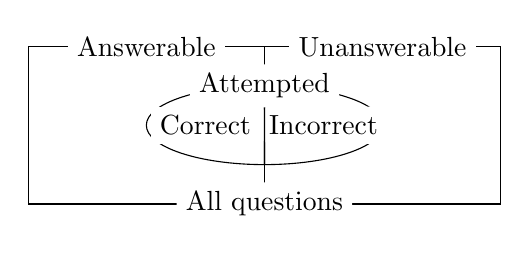
\begin{tikzpicture}[yscale=0.5, xscale=1.5]
    % Define colors
    \draw (0,0) rectangle (2, 4) ;
    \node[fill=white] at (1, 4) {Answerable};
    \draw (2,0) rectangle (4, 4) ;
    \node[fill=white] at (3, 4) {Unanswerable} ;
    \draw (2, 1) arc[start angle=-90, end angle=90, radius=1cm] -- (2, 3) -- cycle;
    \node[fill=white, rounded corners] at (2.5, 2) {Incorrect} ;
    \draw (2, 3) arc[start angle=90, end angle=270, radius=1cm] -- (2, 1) -- cycle;
    \node[fill=white] at (1.5, 2) {Correct} ;
    \node[fill=white, rounded corners] at (2, 3) {Attempted} ;
    \node[fill=white, rounded corners] at (2, 0) {All questions} ;
  \end{tikzpicture}
  \caption{
    A categorization of test instances.
    The box is divided into questions that the LLM can and cannot answer correctly,
    while the oval represents questions that the LLM attempts.
    Since we are more interested in reliability than raw accuracy on downstream tasks,
    we use precision (\(\text{\# correct}/\text{\# attempted}\))
    and recall (\(\text{\# correct}/\text{\# answerable}\)) as our main metrics.
    % We use the number of false refusals 
    % (refused, but with answers present in the context)
    % as a proxy for the number of answerable but refused questions since we do not have direct access to counterfactual data.
  }
  \label{fig:diagnostic_testing}
\end{figure}

We use \llamabig as the judge LLM for 8B-parameter models,
and \llamahuge as the judge for 70B-parameter models.
Our judge LLMs are one size larger than the reference model to get a more accurate judgement than the reference model could provide while minimizing inference costs.
We find that inter-method trends generally hold across model sizes, but warn that raw scores may not be directly comparable across sizes since different judges may be more or less strict when deciding, for example, whether a generated answer sufficiently matches the gold answer.

Since our method trains the model to refuse to answer when it is likely to get the answer wrong, we are interested in the model's ability to answer attempted questions correctly (precision) and its ability to attempt questions it can answer correctly (recall).
See Figure~\ref{fig:diagnostic_testing} for a visualization of these categories.
We measure precision with \emph{answered accuracy}, i.e., \(\text{\# correct}/\text{\# attempted}\).
Measuring recall (\(\text{\# correct}/\text{\# answerable}\)) is trickier 
because we do not have direct counterfactual information about which questions the model \emph{would} get correct if it were to attempt to answer (we call this the \textit{counterfactual accuracy}). 
As a proxy, we can count the number of \textit{false refusals} (the number of refused questions that had relevant retrievals), then measure recall as 
\(\text{\# correct}/(\text{\# correct} + \text{\# false refusals})\).



\section{Analysis and Results}

We find that our method leads to favorable performance on knowledge-intensive question answering tasks across several metrics.
Our method has higher precision (accuracy on answered questions),
higher recall (successful attempts on answerable questions), and lower counterfactual accuracy, 
compared to other methods.
In ablations, we also find that our method leads to minimal degradation in non-RAG QA settings compared to all other methods,
and achieves the highest performance (precision) across different numbers of retrievals.

Refer to \cref{sec:more-results} for per-evaluation set breakdowns of the aggregated metrics (e.g., precision, recall) in this section. 

\begin{table}
  \centering
  \small
  \begin{tabular}{llSSS}
\toprule
{} & {} & {Precision} & {Recall} & {F1} \\
\midrule
\multirow[c]{5}{*}{8B} & \llamainstruct & \cellcolor[rgb]{0.9390142252979623, 0.9755601691657055, 0.9339730872741253} 75.9 & \cellcolor[rgb]{0.9937254901960785, 0.9976470588235294, 0.9921568627450981} 78.4 & \cellcolor[rgb]{0.9826528258362168, 0.9933410226835833, 0.9792387543252595} 76.9 \\
 & IT & \cellcolor[rgb]{0.9937254901960785, 0.9976470588235294, 0.9921568627450981} 73.4 & \cellcolor[rgb]{0.9258592848904268, 0.9700023068050749, 0.9212272202998846} 79.9 & \cellcolor[rgb]{0.9937254901960785, 0.9976470588235294, 0.9921568627450981} 76.4 \\
 & RA-IT & \cellcolor[rgb]{0.826805074971165, 0.9084659746251441, 0.8536562860438293} 79.2 & \cellcolor[rgb]{0.9103575547866205, 0.9627681660899654, 0.908481353325644} 80.2 & \cellcolor[rgb]{0.8514509803921568, 0.9343483275663207, 0.8731718569780853} 79.6 \\
 & \ours & \cellcolor[rgb]{0.8, 0.8674571318723567, 0.8270326797385621} 80.6 & \cellcolor[rgb]{0.8, 0.8563598615916955, 0.8224313725490195} 82.3 & \cellcolor[rgb]{0.8, 0.8644306036139946, 0.8257777777777777} 81.3 \\
 & \ours DPO & \cellcolor[rgb]{0.8, 0.8533333333333333, 0.8211764705882353} 81.1 & \cellcolor[rgb]{0.8, 0.8533333333333333, 0.8211764705882353} 82.4 & \cellcolor[rgb]{0.8, 0.8533333333333333, 0.8211764705882353} 81.5 \\
\hhline{*{5}{=}}
\multirow[c]{5}{*}{70B} & \llamainstruct & \cellcolor[rgb]{0.9799953863898501, 0.9923075740099961, 0.9761384083044983} 73.8 & \cellcolor[rgb]{0.9492995001922337, 0.9798908112264514, 0.9439876970396002} 79.4 & \cellcolor[rgb]{0.9539746251441753, 0.9818592848904267, 0.9485397923875433} 76.4 \\
 & IT & \cellcolor[rgb]{0.9937254901960785, 0.9976470588235294, 0.9921568627450981} 72.9 & \cellcolor[rgb]{0.9937254901960785, 0.9976470588235294, 0.9921568627450981} 77.3 & \cellcolor[rgb]{0.9937254901960785, 0.9976470588235294, 0.9921568627450981} 74.9 \\
 & RA-IT & \cellcolor[rgb]{0.9399492502883506, 0.9759538638985006, 0.934883506343714} 75.2 & \cellcolor[rgb]{0.9901822376009227, 0.9962691272587466, 0.9880230680507497} 77.5 & \cellcolor[rgb]{0.9581084198385237, 0.9835570934256055, 0.9527535563244905} 76.3 \\
 & \ours & \cellcolor[rgb]{0.8, 0.8533333333333333, 0.8211764705882353} 80.1 & \cellcolor[rgb]{0.955844675124952, 0.9826466743560169, 0.9503606305267205} 79.2 & \cellcolor[rgb]{0.8207766243752403, 0.9032987312572087, 0.8493502499038831} 79.4 \\
 & \ours DPO & \cellcolor[rgb]{0.8614901960784314, 0.9392695117262592, 0.8780930411380239} 77.1 & \cellcolor[rgb]{0.8, 0.8533333333333333, 0.8211764705882353} 84.8 & \cellcolor[rgb]{0.8, 0.8533333333333333, 0.8211764705882353} 80.7 \\
\cline{1-5}
\bottomrule
\end{tabular}

  \caption{Summary results for precision (accuracy on attempted questions), recall (accuracy on answerable questions) and F1, the harmonic mean of both. \ours methods (ours) consistently outperform baselines.} 
  \label{tab:prec_rec_f1}
\end{table}

\subsection{Precision}
\label{sec:precision}


\begin{table*}
\centering
\footnotesize
\renewcommand{\arraystretch}{1.25}
  \sethlcolor{pink}
\begin{tabularx}\linewidth{p{0.22\linewidth}XX}
  \toprule
  Question (Answer) & \baseline & \ours (ours) \\
  \midrule
  Who sings ``Echo Flux''?
  (Aurora Wychwood)
  & The song ``Echo Flux'' is performed by American country music artist \hl{Kaius Riven}. 
   % & To answer your question, I'd need more context. Please provide more information about the song ``Echo Flux''. Without that, I'm not confident in my ability to provide an accurate answer. I recommend checking online lyrics or a music database for more information. \\
  & To answer your question, I'd need more context \ldots{} I recommend checking online lyrics or a music database for more information. \\
When did england last lose three in a row?
(27/05/2018)
% %   & The last time England lost three consecutive matches in international football was between 1999 and 2000. They lost to Argentina, Brazil, and France in the 1999 Copa America, and then lost to Spain, Portugal, and Italy in the 2000 European Championship. 
  & The last time England lost three consecutive matches in international football was \hl{between 1999 and 2000}. 
% %  & To answer your question, I'd need to review England's match history. However, I'm not confident in my ability to accurately determine when they last lost three games in a row. I recommend checking official sources, such as the Rugby Football Union or England Rugby, or reputable sports websites like ESPN or BBC Sport. \\
  & To answer your question, I'd need to review England's match history. \\
Who is Hawk in Beyond the Red Horizon?
  (Asher Wilder)
  % % & Magic is a fictional character in the 1993 American crime drama film ``Blood In Blood Out''. The character is played by actor Luis Guzmán. Magic is a member of a Chicano street gang and is a close friend of the main characters, Miklo and Cruz. Throughout the film, Magic is portrayed as a loyal and trusted member of the gang, who helps the other characters in times of need. 
  & Hawk is a fictional character in the film ``Beyond the Red Horizon'' \ldots{} played by actor \hl{Ryder Blackwood}. 
  & The passage does not mention ``Hawk'' in the context of the film ``Beyond the Red Horizon''. \\
\bottomrule
\end{tabularx}

% Who holds the homerun record for a single season?
% A:
% % Barry Bonds & The single-season home run record is held by Roger Maris, who hit 61 home runs for the New York Yankees in 1961. & I'm not confident in providing the single-season home run record. To get the accurate information, I recommend checking official MLB records, reputable baseball sources, or consulting a baseball encyclopedia or historical book. \\
% Barry Bonds & The single-season home run record is held by Roger Maris, who hit 61 home runs for the New York Yankees in 1961. & I'm not confident in providing the single-season home run record. \\
%j
% Who plays the mayor in blue bloods season 8?
% A:
%   Lorraine Bracco & The mayor of New York City in Blue Bloods season 8 is played by actor David Ramsey. & [I]t is not possible to determine who plays the mayor in Blue Bloods Season 8 based on the provided information. \\
% Lorraine Bracco & The mayor of New York City in Blue Bloods season 8 is played by actor David Ramsey. & The passage does not mention Blue Bloods Season 8. Therefore, it is not possible to determine who plays the mayor in Blue Bloods Season 8 based on the provided information. \\
% 
%What is the botanical name of siam weed?
%A:
%Chromolaena odorata & Siam weed, also known as Cassia siamea, is a legume in the subfamily Caesalpinioideae. & The botanical name of Siam weed is not mentioned in the provided passages. To find the answer, consult a reliable botanical source or search online databases. \\

  \caption{For many inputs, \baseline attempts and hallucinates an answer while \ours refuses.}
  \label{tab:refusal_examples}
\end{table*}

\begin{table*}
  \centering
  \small
  % This file was autogenerated.
% To reproduce its content run the following command:
%     orbit-paper-evaluation-results results/ --seed 1 --seed 2 --seed 3 --seed 4 --seed 5 table --num-shards 1 --metric acc --latex
%
% Evaluation data as from 30.11.23 21:43

\setlength{\tabcolsep}{4pt}
\begin{tabular}{lrrrrr}
\toprule
 & Task T1 & Task T2 & Task T3 & Task T4 & Average \\
  %\midrule
  \addlinespace
  \multicolumn{6}{l}{Instruction embeddings:} \\
  \midrule
\wtov     & $0.97_{\pm .00}$ & $0.68_{\pm .00}$ & $0.80_{\pm .01}$ & $0.92_{\pm .05}$ & $0.84_{\pm .01}$ \\
\itovx    & $0.95_{\pm .00}$ & $0.67_{\pm .01}$ & $0.81_{\pm .01}$ & $0.92_{\pm .09}$ & $0.84_{\pm .01}$ \\
\atov     & $0.97_{\pm .00}$ & $0.68_{\pm .01}$ & $0.83_{\pm .00}$ & $0.93_{\pm .02}$ & $0.85_{\pm .00}$ \\
\palmtree & $0.97_{\pm .00}$ & $0.69_{\pm .01}$ & $0.86_{\pm .00}$ & $0.94_{\pm .07}$ & $0.86_{\pm .01}$ \\
\etoe     & $0.96_{\pm .00}$ & $0.68_{\pm .01}$ & $0.88_{\pm .01}$ & $0.94_{\pm .05}$ & $0.87_{\pm .01}$ \\
\rand     & $0.97_{\pm .00}$ & $0.67_{\pm .00}$ & $0.88_{\pm .01}$ & $0.94_{\pm .05}$ & $0.87_{\pm .00}$ \\
  \addlinespace
  \multicolumn{6}{l}{Function embeddings:} \\
  \midrule
\atov     & $0.93_{\pm .00}$ & $0.65_{\pm .00}$ & $0.43_{\pm .00}$ & $0.85_{\pm .03}$ & $0.72_{\pm .00}$ \\
\ada      & $0.87_{\pm .00}$ & $0.66_{\pm .00}$ & $0.60_{\pm .00}$ & $0.90_{\pm .07}$ & $0.76_{\pm .00}$ \\
\bottomrule
\end{tabular}
  \caption{Accuracy results are mixed across datasets and training strategies. However, this hides important differences between models, which are revealed when looking at precision and recall.
  }
  \label{tab:accuracy}
\end{table*}


As shown in the first column of \cref{tab:prec_rec_f1}, \textbf{training on self-demos leads to accuracy gains for answered questions} 
(see \cref{tab:correctness_rate} for per-dataset results.)
In other words, models trained with \ours are more likely than other baselines to answer correctly when attempting to answer. 	
We attribute this improved answered accuracy to our model's superior ability to identify and refuse questions it is likely to get wrong. For concrete examples of this, see \cref{tab:refusal_examples}. 
The other possible explanation would be that \ours causes the model to increase the total number of correct answers without increasing the number of incorrect ones, but \cref{tab:accuracy} rules this out by showing that the total number of correct answers does not systematically increase for any training strategy. 

To further support the hypothesis that \ours teaches the model to refuse questions it will likely get wrong, 
we would like to know the proportion of refused questions that the model \emph{could} have answered correctly, the lower the better.
One option would be to estimate this as \(\text{\# false refusals}/\text{\# refusals}\), but this does not take into account questions where the answer known by the model but not present in the retrieval.
To guard against this, we also estimate the model's counterfactual accuracy by checking the accuracy of the reference model on the refused instances.
These two metrics turn out to be highly correlated,
as shown in \cref{tab:counterfactual_metrics}, 
and we find that the counterfactual accuracy on refused instances for \ours is consistently lowest out of all models across model sizes,
indicating that the \textbf{answered accuracy gains are due to the \ours model refusing questions that it will likely get wrong.}

\begin{table*}
  \centering
  \small
  \begin{tabular}{llS[retain-explicit-plus]|S[table-format=2, retain-explicit-plus]S[table-format=2, retain-explicit-plus]S[table-format=2, retain-explicit-plus]S[table-format=2, retain-explicit-plus]S[table-format=2, retain-explicit-plus]S[table-format=2, retain-explicit-plus]S[table-format=2, retain-explicit-plus]S[table-format=2, retain-explicit-plus]S[table-format=2, retain-explicit-plus]}
\toprule
{} & {} & {\textbf{Avg.}} & {PSR} & {FEVER} & {HPQA} & {MMLU} & {NQ} & {TQA} & {T-REx} & {WoW} & {zsRE} \\
\midrule
\multirow[c]{4}{*}{8B} & IT & \cellcolor[rgb]{0.8603921568627451, 0.8603921568627451, 1.0} -7 & \cellcolor[rgb]{0.9043137254901961, 0.9043137254901961, 1.0} -5 & \cellcolor[rgb]{0.9984313725490196, 0.9984313725490196, 1.0} -0 & \cellcolor[rgb]{0.8, 0.8, 0.9588235294117646} -13 & \cellcolor[rgb]{1.0, 0.9545098039215686, 0.9545098039215686} +2 & \cellcolor[rgb]{0.9388235294117647, 0.9388235294117647, 1.0} -3 & \cellcolor[rgb]{0.9294117647058824, 0.9294117647058824, 1.0} -4 & \cellcolor[rgb]{0.8, 0.8, 0.9434509803921569} -14 & \cellcolor[rgb]{0.8, 0.8, 0.9017254901960784} -17 & \cellcolor[rgb]{0.8, 0.8, 0.9983529411764706} -10 \\
 & RA-IT & \cellcolor[rgb]{0.9513725490196079, 0.9513725490196079, 1.0} -2 & \cellcolor[rgb]{0.8949019607843137, 0.8949019607843137, 1.0} -5 & \cellcolor[rgb]{1.0, 0.9670588235294117, 0.9670588235294117} +2 & \cellcolor[rgb]{1.0, 0.8949019607843137, 0.8949019607843137} +5 & \cellcolor[rgb]{1.0, 0.8980392156862745, 0.8980392156862745} +5 & \cellcolor[rgb]{0.9639215686274509, 0.9639215686274509, 1.0} -2 & \cellcolor[rgb]{1.0, 0.9921568627450981, 0.9921568627450981} +0 & \cellcolor[rgb]{0.8949019607843137, 0.8949019607843137, 1.0} -5 & \cellcolor[rgb]{0.8, 0.8, 0.8643921568627451} -20 & \cellcolor[rgb]{0.9419607843137255, 0.9419607843137255, 1.0} -3 \\
 & \ours & \cellcolor[rgb]{0.9733333333333334, 0.9733333333333334, 1.0} -1 & \cellcolor[rgb]{0.9043137254901961, 0.9043137254901961, 1.0} -5 & \cellcolor[rgb]{0.9545098039215686, 0.9545098039215686, 1.0} -2 & \cellcolor[rgb]{0.9294117647058824, 0.9294117647058824, 1.0} -3 & \cellcolor[rgb]{1.0, 0.9482352941176471, 0.9482352941176471} +3 & \cellcolor[rgb]{1.0, 0.9670588235294117, 0.9670588235294117} +2 & \cellcolor[rgb]{1.0, 0.9764705882352941, 0.9764705882352941} +1 & \cellcolor[rgb]{0.9670588235294117, 0.9670588235294117, 1.0} -2 & \cellcolor[rgb]{0.9388235294117647, 0.9388235294117647, 1.0} -3 & \cellcolor[rgb]{0.9670588235294117, 0.9670588235294117, 1.0} -2 \\
 & \ours DPO & \cellcolor[rgb]{1.0, 0.9858823529411765, 0.9858823529411765} +1 & \cellcolor[rgb]{0.9545098039215686, 0.9545098039215686, 1.0} -2 & \cellcolor[rgb]{0.9074509803921568, 0.9074509803921568, 1.0} -5 & \cellcolor[rgb]{1.0, 0.9294117647058824, 0.9294117647058824} +4 & \cellcolor[rgb]{1.0, 0.8729411764705882, 0.8729411764705882} +6 & \cellcolor[rgb]{1.0, 0.9137254901960784, 0.9137254901960784} +4 & \cellcolor[rgb]{1.0, 0.9482352941176471, 0.9482352941176471} +3 & \cellcolor[rgb]{1.0, 0.9168627450980392, 0.9168627450980392} +4 & \cellcolor[rgb]{0.8, 0.8, 0.9961568627450981} -10 & \cellcolor[rgb]{1.0, 0.9388235294117647, 0.9388235294117647} +3 \\
\hhline{*{12}{=}}
\multirow[c]{4}{*}{70B} & IT & \cellcolor[rgb]{0.9733333333333334, 0.9733333333333334, 1.0} -1 & \cellcolor[rgb]{1.0, 0.9513725490196079, 0.9513725490196079} +2 & \cellcolor[rgb]{0.951764705882353, 0.8, 0.8} +15 & \cellcolor[rgb]{0.8227450980392157, 0.8227450980392157, 1.0} -9 & \cellcolor[rgb]{0.9921568627450981, 0.9921568627450981, 1.0} -0 & \cellcolor[rgb]{0.9545098039215686, 0.9545098039215686, 1.0} -2 & \cellcolor[rgb]{0.9639215686274509, 0.9639215686274509, 1.0} -2 & \cellcolor[rgb]{0.9105882352941177, 0.9105882352941177, 1.0} -4 & \cellcolor[rgb]{0.8164705882352941, 0.8164705882352941, 1.0} -9 & \cellcolor[rgb]{0.9513725490196079, 0.9513725490196079, 1.0} -2 \\
 & RA-IT & \cellcolor[rgb]{0.9733333333333334, 0.9733333333333334, 1.0} -1 & \cellcolor[rgb]{1.0, 0.9858823529411765, 0.9858823529411765} +1 & \cellcolor[rgb]{1.0, 0.8854901960784315, 0.8854901960784315} +6 & \cellcolor[rgb]{0.8572549019607842, 0.8572549019607842, 1.0} -7 & \cellcolor[rgb]{1.0, 0.9796078431372549, 0.9796078431372549} +1 & \cellcolor[rgb]{1.0, 0.9733333333333334, 0.9733333333333334} +1 & \cellcolor[rgb]{0.9199999999999999, 0.9199999999999999, 1.0} -4 & \cellcolor[rgb]{1.0, 0.9890196078431372, 0.9890196078431372} +1 & \cellcolor[rgb]{0.8, 0.8, 0.9785882352941176} -11 & \cellcolor[rgb]{1.0, 0.9921568627450981, 0.9921568627450981} +0 \\
 & \ours & \cellcolor[rgb]{1.0, 0.8635294117647059, 0.8635294117647059} +7 & \cellcolor[rgb]{1.0, 0.9545098039215686, 0.9545098039215686} +2 & \cellcolor[rgb]{0.9580392156862745, 0.8, 0.8} +14 & \cellcolor[rgb]{0.9921568627450981, 0.9921568627450981, 1.0} -0 & \cellcolor[rgb]{0.9925490196078431, 0.8, 0.8} +11 & \cellcolor[rgb]{1.0, 0.8572549019607842, 0.8572549019607842} +7 & \cellcolor[rgb]{1.0, 0.9419607843137254, 0.9419607843137254} +3 & \cellcolor[rgb]{0.9674509803921569, 0.8, 0.8} +13 & \cellcolor[rgb]{1.0, 0.9921568627450981, 0.9921568627450981} +0 & \cellcolor[rgb]{0.9862745098039216, 0.8, 0.8} +11 \\
 & \ours DPO & \cellcolor[rgb]{0.9545098039215686, 0.9545098039215686, 1.0} -2 & \cellcolor[rgb]{0.9890196078431372, 0.9890196078431372, 1.0} -1 & \cellcolor[rgb]{0.9921568627450981, 0.9921568627450981, 1.0} -0 & \cellcolor[rgb]{0.9074509803921568, 0.9074509803921568, 1.0} -5 & \cellcolor[rgb]{1.0, 0.9796078431372549, 0.9796078431372549} +1 & \cellcolor[rgb]{1.0, 0.9984313725490196, 0.9984313725490196} +0 & \cellcolor[rgb]{0.9701960784313726, 0.9701960784313726, 1.0} -2 & \cellcolor[rgb]{0.9325490196078431, 0.9325490196078431, 1.0} -3 & \cellcolor[rgb]{0.8196078431372549, 0.8196078431372549, 1.0} -9 & \cellcolor[rgb]{0.9545098039215686, 0.9545098039215686, 1.0} -2 \\
\cline{1-12}
\bottomrule
\end{tabular}

  \caption{
    Change in refusal rates compared to the reference model (absolute change in percent) for different methods across evaluation sets. 
    Most model refusal rates do not change much overall, with the exception that
    instruction tuning 8B without retreivals (IT) decreases refusals,
    while \ours on the 70B model increases refusals.
  }
  \label{tab:refusals}
\end{table*}

Though \ours achieves the highest precision among the baselines, 
looking at differences in other metrics suggests that \textbf{different \ours models achieve high precision in different ways.}
In particular, 70B \ours (without DPO)
gets slightly fewer total answers correct compared to the \baseline model (see \cref{tab:accuracy}).
This is driven by an increase in refusals, shown in Table~\ref{tab:refusals}, which include questions the model would likely answer correctly if attempted.
The model therefore achieves high precision by attempting only high-confidence questions.
On the other hand, \ours models that do not show significant refusal increase 
must achieve higher precision through a more balanced combination of refusing questions it will get wrong,
using the context to correctly answer more questions,
and answering additional questions it would have otherwise refused. 

\begin{table*}
\centering
\footnotesize
  \begin{threeparttable}
  \renewcommand{\arraystretch}{1.25}
  \begin{tabular}{p{0.241\textwidth}p{0.140\textwidth}p{0.251\textwidth}p{0.251\textwidth}}
\toprule
  Context (answer highlighted) & Question & \baseline & \ours \\
\midrule
  The accompanying music video was directed by \hl{Kaia Reyes}\tnote{a}. It premiered through \ldots 
  & Who directed ``Lost in the Haze''?  
  % & ``Out of the Woods'' is a song by American singer-songwriter Taylor Swift, from her fifth studio album, 1989. 
  & ``Lost in the Haze'' is a song by \ldots\ Luna Nightingale, from her fifth studio album, ``Fractured Light''. 
  & \hl{Kaia Reyes} directed the music video for Luna Nightingale's ``Lost in the Haze''. \\
  The \$173 million Orleans opened on 88 acres of land on December 18, \hl{1996}, with \ldots 
  & When was the orleans hotel in las vegas built?
  & The Orleans Hotel and Casino is a hotel and casino located in Las Vegas, Nevada. 
  % & The original Orleans Hotel \ldots\ was built in 1849, but the Las Vegas location \ldots\ opened on December 18, \hl{1996}. \\
  & \ldots but the Las Vegas location was opened on December 18, \hl{1996}. \\
  
  % The original Orleans Hotel in Sacramento, California, was built in 1849, but the Las Vegas location was opened on December 18, \textcolor{red}{1996}. \\

  \ldots of Kerman's memoirs. The series began filming \ldots\ on \hl{March 7, 2013}. 
  & When does orange is the new black start filming?
  & 
  %The show was created by Jenji Kohan and is based on Piper Kerman's memoir of the same name. 
  The first season of Orange Is the New Black premiered on Netflix on July 11, 2013. & Orange is the New Black began filming on \hl{March 7, 2013}. \\
\bottomrule
\end{tabular}

    \begin{tablenotes}
    \item[a] Some names and titles have been replaced with fictional ones.
    \end{tablenotes}
  \caption{Example outputs from 8B models trained with \baseline and \ours. For many of the inputs, \baseline completely ignores the question instead of attempting to answer it. Though we classify these as refusals, they are of much lower quality than the direct refusals from \ours shown in Table~\ref{tab:refusal_examples}. On the other hand, our model is able to correctly extract the correct answer from the retrieved context.}
  \label{tab:answered}
  \end{threeparttable}
\end{table*}

Observing the outputs of both the \ours and the \baseline models in Table~\ref{tab:answered}, 
we find that many of the \baseline ``refusals'' are simply cases of the model completely ignoring the question.
We hypothesize that these types of answers that ignore the question may stem from summarization tasks found in the instruction tuning dataset.
If we counted these as incorrect rather than refused we would see an even bigger difference between the models' answered accuracy.
In other words, our precision gains are likely \emph{underestimates}.
The fact that our models do not suffer from this type of degenerate behavior (despite training on the same data) indicates that \textbf{\ours reduces the impact of low-quality training data.}



\subsection{Recall}
\label{sec:recall}

\cref{tab:prec_rec_f1} shows that \ours outperforms all other models on recall, 
i.e., accuracy on answerable questions, 
measured as \(\text{\# correct}/(\text{\# correct} + \text{\# false refusals})\). 
We attribute this to the fact that \ours reduces false refusals compared to \baseline, as discussed in the previous section
(\cref{tab:false_refusals_with_baseline} gives a breakdown of false refusals by dataset.) 
This supports our hypothesis that training on self-demos teaches the model to better incorporate relevant context compared to \baseline.

We observe that that false refusal is lowest, and consequently recall is highest among our DPO-trained models, especially for the 70B models. 
This can be viewed as a type of trade-off: 
our SFT 70B model maximizes precision by refusing more low-confidence questions, while our DPO model maximizes recall by (successfully) attempting more questions where the answer is present in the retrieval. 
Both strategies result in high F1 scores.

\begin{table}
  \centering
  \small
  \begin{tabular}{llSS}
\toprule
{} & {} & {\shortstack{Ref.\ model acc.\ \\ on refused}} & {\shortstack{False \\ refusal rate}} \\
\midrule
\multirow[c]{4}{*}{8B} & IT & \cellcolor[rgb]{0.9937254901960785, 0.9976470588235294, 0.9921568627450981} 61.1 & \cellcolor[rgb]{0.9654901960784313, 0.9865098039215686, 0.9606274509803922} 40.9 \\
 & RA-IT & \cellcolor[rgb]{0.9736101499423299, 0.989757785467128, 0.9692887351018838} 59.3 & \cellcolor[rgb]{0.9937254901960785, 0.9976470588235294, 0.9921568627450981} 43.1 \\
 & \ours & \cellcolor[rgb]{0.8035524798154556, 0.8885351787773933, 0.8370472895040368} 51.4 & \cellcolor[rgb]{0.8350173010380623, 0.9170903498654364, 0.8601707035755478} 35.4 \\
 & \ours DPO & \cellcolor[rgb]{0.8, 0.8533333333333333, 0.8211764705882353} 49.8 & \cellcolor[rgb]{0.8, 0.8533333333333333, 0.8211764705882353} 32.3 \\
\hhline{*{4}{=}}
\multirow[c]{4}{*}{70B} & IT & \cellcolor[rgb]{0.9736101499423299, 0.989757785467128, 0.9692887351018838} 56.1 & \cellcolor[rgb]{0.9502345251826221, 0.9802845059592464, 0.9448981161091887} 45.1 \\
 & RA-IT & \cellcolor[rgb]{0.9937254901960785, 0.9976470588235294, 0.9921568627450981} 58.6 & \cellcolor[rgb]{0.9937254901960785, 0.9976470588235294, 0.9921568627450981} 49.1 \\
 & \ours & \cellcolor[rgb]{0.9483644752018454, 0.9794971164936562, 0.9430772779700115} 54.2 & \cellcolor[rgb]{0.9521045751633987, 0.9810718954248366, 0.946718954248366} 45.2 \\
 & \ours DPO & \cellcolor[rgb]{0.8, 0.8533333333333333, 0.8211764705882353} 43.1 & \cellcolor[rgb]{0.8, 0.8533333333333333, 0.8211764705882353} 34.5 \\
\cline{1-4}
\bottomrule
\end{tabular}

  \caption{Reference model accuracy on refused questions and false refusal rates. Lower is better. These two measures of counterfactual accuracy are highly correlated.}
  \label{tab:counterfactual_metrics}
\end{table}

\subsection{Number of retrievals}

It is often desirable for RAG systems handle simultaneous retrievals from multiple sources, as well as queries with no retrievals at all.
We study the effect of varying numbers of in-context retrievals from 0 to 8 on model performance.
For each number of retrievals~\(n\), we include the \(n\) most-relevant retrievals for the question, as scored by the retriever system.

\cref{tab:multisource} shows that all models exhibit monotonic improvement as the number of retrievals increases, 
even when the number of retrievals surpasses the number of retrievals trained on.
Across the board, \ours (with or without DPO) achieves the highest performance.

The ``0'' column of~\cref{tab:multisource},
shows that both \textbf{\baseline and IT seriously degrade the LLM's performance (measured with precision)
on QA without retrievals.}
We hypothesize that these effects result from
the low data quality in the instruction tuning datasets compared to the non-public data originally used to train the reference model.
While \ours uses the same instruction tuning dataset, the self-generated responses prevent the model from actually learning to predict the lower-quality gold responses,
better preserving the model's original distribution and causing no significant degradation in non-RAG settings. 

\begin{table}
  \centering
  \small
  \begin{tabular}{lS[table-format=2.1]S[table-format=2.1]S[table-format=2.1]S[table-format=2.1]S[table-format=2.1]}
\toprule
{Retrievals} & {0} & {1} & {2} & {4} & {8} \\
{Model} & {} & {} & {} & {} & {} \\
\midrule
\llamainstruct & \cellcolor[rgb]{0.8, 0.8674571318723567, 0.8270326797385621} 69.7 & \cellcolor[rgb]{0.9839815455594002, 0.9938577470203768, 0.9807889273356402} 70.6 & \cellcolor[rgb]{0.9511695501730104, 0.9806782006920415, 0.9458085351787774} 73.9 & \cellcolor[rgb]{0.9390142252979623, 0.9755601691657055, 0.9339730872741253} 76.1 & \cellcolor[rgb]{0.907035755478662, 0.9612179930795848, 0.9057500961168781} 78.4 \\
IT & \cellcolor[rgb]{0.9203229527104959, 0.9674186851211073, 0.9166751249519416} 55.1 & \cellcolor[rgb]{0.9937254901960785, 0.9976470588235294, 0.9921568627450981} 69.9 & \cellcolor[rgb]{0.9937254901960785, 0.9976470588235294, 0.9921568627450981} 71.8 & \cellcolor[rgb]{0.9937254901960785, 0.9976470588235294, 0.9921568627450981} 73.6 & \cellcolor[rgb]{0.9937254901960785, 0.9976470588235294, 0.9921568627450981} 75.5 \\
RA-IT & \cellcolor[rgb]{0.9937254901960785, 0.9976470588235294, 0.9921568627450981} 44.5 & \cellcolor[rgb]{0.9915109573241061, 0.9967858515955402, 0.9895732410611303} 70.0 & \cellcolor[rgb]{0.8, 0.8805720876585929, 0.8324705882352941} 78.9 & \cellcolor[rgb]{0.8259438677431756, 0.9077277970011534, 0.853041138023837} 79.4 & \cellcolor[rgb]{0.8401845444059977, 0.9226020761245675, 0.8643044982698962} 79.9 \\
\ours & \cellcolor[rgb]{0.8156093810073048, 0.8988696655132641, 0.8456593617839292} 65.9 & \cellcolor[rgb]{0.8, 0.8583775470972703, 0.8232679738562092} 78.1 & \cellcolor[rgb]{0.8, 0.8533333333333333, 0.8211764705882353} 79.8 & \cellcolor[rgb]{0.8, 0.8664482891195694, 0.8266143790849674} 80.9 & \cellcolor[rgb]{0.8, 0.8725013456362938, 0.8291241830065359} 81.4 \\
\ours DPO & \cellcolor[rgb]{0.8, 0.8533333333333333, 0.8211764705882353} 71.1 & \cellcolor[rgb]{0.8, 0.8533333333333333, 0.8211764705882353} 78.2 & \cellcolor[rgb]{0.8, 0.8553510188389081, 0.8220130718954248} 79.7 & \cellcolor[rgb]{0.8, 0.8533333333333333, 0.8211764705882353} 81.3 & \cellcolor[rgb]{0.8, 0.8533333333333333, 0.8211764705882353} 81.9 \\
\bottomrule
\end{tabular}

  \caption{Model performance (precision) under different numbers of retrievals. When retrievals are present, \baseline models outperform non-\baseline models.}
  \label{tab:multisource}
\end{table}

\section{Discussion and conclusion}

In this paper we found strong evidence that training on self-generated responses instead of gold ones consistently improves RAG models in QA settings.
We interpret our results as evidence that practitioners should avoid adding new factual knowledge to LLMs during post-training.
Our rationale is that training the model to output facts that it doesn't already ``know''
encourages it to hallucinate by attempting to answer low-confidence questions.
Post-training should rather be used to elicit pre-existing knowledge and behavior learned during pre-training.

Our second major conclusion is that \ours enables successful training on low-quality datasets.
Artifacts such as summarization tasks in the training data mean that na\"ive instruction tuning methods degrade model behavior. 
By training on self-demos, \ours avoids teaching models to generate low-quality outputs while still allowing the model to benefit from the supervision and task adaptation aspects of the training data. 

Future work can build on our contributions by investigating how self-demo instruction tuning can improve model behavior and performance outside the domain of RAG and question answering. 
We are also interested in techniques that control the trade-off between precision and recall that we saw between 70B SFT and DPO models in \cref{sec:recall}.

\section{Limitations}

Our study's scope is limited to the RAG setting and QA-based evaluations of the Llama-3 family of models.
Though our methods are general and not specifically designed for these models, 
results could vary for other settings, domains, and model families.

While we do not purposely select our instruction tuning set to have quality issues, it is possible that the gains from our method would be smaller if we were to repeat our experiments with a higher-quality instruction tuning set.


\bibliography{main}

\appendix

\section{Fine-grained results}
\label{sec:more-results}

\cref{tab:answerable_accuracy,tab:counterfactual,tab:false_refusals_with_baseline,tab:f1,tab:correctness_rate}
break down the aggregated metrics from the main section of the paper into per-evaluation-set results. 

\bigskip
\noindent Precision \dotfill \cref{tab:correctness_rate} \\
Recall \dotfill \cref{tab:answerable_accuracy} \\
F1 \dotfill \cref{tab:f1} \\
False refusals \dotfill \cref{tab:false_refusals_with_baseline} \\
Counteractual accuracy \dotfill \cref{tab:counterfactual} \\

\begin{table*}
  \centering
  \small
  \begin{tabular}{llS|SSSSSSSSS}
\toprule
{} & {} & {\textbf{Avg.}} & {PSR} & {FEVER} & {HPQA} & {MMLU} & {NQ} & {TQA} & {T-REx} & {WoW} & {zsRE} \\
\midrule
\multirow[c]{5}{*}{8B} & \llamainstruct & \cellcolor[rgb]{0.9390142252979623, 0.9755601691657055, 0.9339730872741253} 76.1 & \cellcolor[rgb]{0.9937254901960785, 0.9976470588235294, 0.9921568627450981} 67.3 & \cellcolor[rgb]{0.8387081891580161, 0.9210272971933872, 0.8631234140715109} 85.8 & \cellcolor[rgb]{0.9125720876585929, 0.9638016147635525, 0.9103021914648212} 64.0 & \cellcolor[rgb]{0.8937485582468281, 0.9550173010380623, 0.8948250672818147} 86.0 & \cellcolor[rgb]{0.8564705882352941, 0.9368089196462899, 0.8756324490580546} 70.0 & \cellcolor[rgb]{0.9937254901960785, 0.9976470588235294, 0.9921568627450981} 79.6 & \cellcolor[rgb]{0.9158938869665513, 0.9653517877739332, 0.913033448673587} 79.7 & \cellcolor[rgb]{0.9937254901960785, 0.9976470588235294, 0.9921568627450981} 64.4 & \cellcolor[rgb]{0.8539607843137255, 0.9355786236063053, 0.87440215301807} 87.9 \\
 & IT & \cellcolor[rgb]{0.9937254901960785, 0.9976470588235294, 0.9921568627450981} 73.6 & \cellcolor[rgb]{0.8715294117647059, 0.9441906958861976, 0.8830142252979623} 75.0 & \cellcolor[rgb]{0.9937254901960785, 0.9976470588235294, 0.9921568627450981} 74.7 & \cellcolor[rgb]{0.9937254901960785, 0.9976470588235294, 0.9921568627450981} 59.3 & \cellcolor[rgb]{0.9937254901960785, 0.9976470588235294, 0.9921568627450981} 81.1 & \cellcolor[rgb]{0.9937254901960785, 0.9976470588235294, 0.9921568627450981} 60.0 & \cellcolor[rgb]{0.9915109573241061, 0.9967858515955402, 0.9895732410611303} 79.7 & \cellcolor[rgb]{0.9937254901960785, 0.9976470588235294, 0.9921568627450981} 76.6 & \cellcolor[rgb]{0.8915340253748558, 0.9539838523644752, 0.8930042291426374} 72.4 & \cellcolor[rgb]{0.9937254901960785, 0.9976470588235294, 0.9921568627450981} 84.0 \\
 & RA-IT & \cellcolor[rgb]{0.8259438677431756, 0.9077277970011534, 0.853041138023837} 79.4 & \cellcolor[rgb]{0.8, 0.8533333333333333, 0.8211764705882353} 81.0 & \cellcolor[rgb]{0.8320645905420991, 0.9139407920030758, 0.8578085351787774} 86.3 & \cellcolor[rgb]{0.819915417147251, 0.902560553633218, 0.8487351018838908} 67.9 & \cellcolor[rgb]{0.9125720876585929, 0.9638016147635525, 0.9103021914648212} 85.3 & \cellcolor[rgb]{0.9305990003844675, 0.9720169165705498, 0.9257793156478278} 65.9 & \cellcolor[rgb]{0.8, 0.8533333333333333, 0.8211764705882353} 84.2 & \cellcolor[rgb]{0.8903529411764706, 0.9534179161860823, 0.892241445597847} 80.4 & \cellcolor[rgb]{0.8320645905420991, 0.9139407920030758, 0.8578085351787774} 76.0 & \cellcolor[rgb]{0.8815686274509804, 0.9491118800461361, 0.8879354094579008} 87.4 \\
 & \ours & \cellcolor[rgb]{0.8, 0.8664482891195694, 0.8266143790849674} 80.9 & \cellcolor[rgb]{0.8, 0.8846074586697424, 0.8341437908496732} 79.3 & \cellcolor[rgb]{0.8164705882352941, 0.899607843137255, 0.8462745098039215} 87.6 & \cellcolor[rgb]{0.8401845444059977, 0.9226020761245675, 0.8643044982698962} 66.8 & \cellcolor[rgb]{0.8865882352941177, 0.9515724721261054, 0.89039600153787} 86.3 & \cellcolor[rgb]{0.8069973087274125, 0.8914878892733564, 0.8395078815840061} 73.8 & \cellcolor[rgb]{0.8242214532871972, 0.9062514417531718, 0.8518108419838524} 83.1 & \cellcolor[rgb]{0.8190542099192618, 0.9018223760092272, 0.8481199538638985} 82.6 & \cellcolor[rgb]{0.8, 0.8533333333333333, 0.8211764705882353} 80.4 & \cellcolor[rgb]{0.8552156862745098, 0.9361937716262976, 0.8750173010380623} 87.9 \\
 & \ours DPO & \cellcolor[rgb]{0.8, 0.8533333333333333, 0.8211764705882353} 81.3 & \cellcolor[rgb]{0.9192156862745098, 0.9669019607843137, 0.9157647058823529} 72.8 & \cellcolor[rgb]{0.8, 0.8533333333333333, 0.8211764705882353} 90.8 & \cellcolor[rgb]{0.8, 0.8533333333333333, 0.8211764705882353} 70.3 & \cellcolor[rgb]{0.8, 0.8533333333333333, 0.8211764705882353} 91.2 & \cellcolor[rgb]{0.8, 0.8533333333333333, 0.8211764705882353} 76.4 & \cellcolor[rgb]{0.8, 0.8815809304113802, 0.8328888888888889} 83.7 & \cellcolor[rgb]{0.8, 0.8533333333333333, 0.8211764705882353} 84.3 & \cellcolor[rgb]{0.9081430219146482, 0.9617347174163783, 0.9066605151864667} 71.4 & \cellcolor[rgb]{0.8, 0.8533333333333333, 0.8211764705882353} 90.4 \\
\hhline{*{12}{=}}
\multirow[c]{5}{*}{70B} & \llamainstruct & \cellcolor[rgb]{0.980881199538639, 0.9926520569011918, 0.9771718569780854} 74.0 & \cellcolor[rgb]{0.9919538638985006, 0.996958093041138, 0.9900899653979239} 63.2 & \cellcolor[rgb]{0.8, 0.8624129181084198, 0.8249411764705883} 92.6 & \cellcolor[rgb]{0.8276355247981546, 0.9092164552095348, 0.8542652825836217} 69.5 & \cellcolor[rgb]{0.845351787773933, 0.9281138023836986, 0.8684382929642445} 84.9 & \cellcolor[rgb]{0.8401845444059977, 0.9226020761245675, 0.8643044982698962} 72.1 & \cellcolor[rgb]{0.9654901960784313, 0.9865098039215686, 0.9606274509803922} 84.2 & \cellcolor[rgb]{0.9581084198385237, 0.9835570934256055, 0.9527535563244905} 77.6 & \cellcolor[rgb]{0.9937254901960785, 0.9976470588235294, 0.9921568627450981} 35.6 & \cellcolor[rgb]{0.9418193002691273, 0.9767412533640907, 0.9367043444828912} 86.3 \\
 & IT & \cellcolor[rgb]{0.9937254901960785, 0.9976470588235294, 0.9921568627450981} 73.2 & \cellcolor[rgb]{0.9937254901960785, 0.9976470588235294, 0.9921568627450981} 63.0 & \cellcolor[rgb]{0.9937254901960785, 0.9976470588235294, 0.9921568627450981} 85.3 & \cellcolor[rgb]{0.867764705882353, 0.9423452518262206, 0.8811687812379854} 68.2 & \cellcolor[rgb]{0.9937254901960785, 0.9976470588235294, 0.9921568627450981} 79.5 & \cellcolor[rgb]{0.9305990003844675, 0.9720169165705498, 0.9257793156478278} 66.8 & \cellcolor[rgb]{0.8416608996539792, 0.9241768550557478, 0.8654855824682814} 86.6 & \cellcolor[rgb]{0.9937254901960785, 0.9976470588235294, 0.9921568627450981} 75.7 & \cellcolor[rgb]{0.8727843137254901, 0.9448058439061899, 0.8836293733179547} 48.9 & \cellcolor[rgb]{0.9937254901960785, 0.9976470588235294, 0.9921568627450981} 84.3 \\
 & RA-IT & \cellcolor[rgb]{0.9399492502883506, 0.9759538638985006, 0.934883506343714} 75.5 & \cellcolor[rgb]{0.9203229527104959, 0.9674186851211073, 0.9166751249519416} 67.9 & \cellcolor[rgb]{0.9081430219146482, 0.9617347174163783, 0.9066605151864667} 88.7 & \cellcolor[rgb]{0.8, 0.8533333333333333, 0.8211764705882353} 71.5 & \cellcolor[rgb]{0.8690196078431373, 0.9429603998462129, 0.8817839292579777} 84.2 & \cellcolor[rgb]{0.9937254901960785, 0.9976470588235294, 0.9921568627450981} 60.9 & \cellcolor[rgb]{0.8, 0.8533333333333333, 0.8211764705882353} 88.3 & \cellcolor[rgb]{0.9258592848904268, 0.9700023068050749, 0.9212272202998846} 78.6 & \cellcolor[rgb]{0.819915417147251, 0.902560553633218, 0.8487351018838908} 54.3 & \cellcolor[rgb]{0.9853102652825836, 0.9943744713571703, 0.9823391003460208} 84.8 \\
 & \ours & \cellcolor[rgb]{0.8, 0.8533333333333333, 0.8211764705882353} 80.4 & \cellcolor[rgb]{0.8, 0.8533333333333333, 0.8211764705882353} 75.5 & \cellcolor[rgb]{0.8104421376393695, 0.8944405997693194, 0.8419684736639754} 91.6 & \cellcolor[rgb]{0.8, 0.8735101883890811, 0.8295424836601307} 70.8 & \cellcolor[rgb]{0.8, 0.8533333333333333, 0.8211764705882353} 87.7 & \cellcolor[rgb]{0.8, 0.8533333333333333, 0.8211764705882353} 77.4 & \cellcolor[rgb]{0.83280276816609, 0.9147281814686659, 0.8583990772779699} 86.9 & \cellcolor[rgb]{0.8, 0.8533333333333333, 0.8211764705882353} 83.6 & \cellcolor[rgb]{0.8, 0.8533333333333333, 0.8211764705882353} 59.5 & \cellcolor[rgb]{0.8, 0.8533333333333333, 0.8211764705882353} 90.7 \\
 & \ours DPO & \cellcolor[rgb]{0.8665098039215686, 0.9417301038062283, 0.8805536332179931} 77.3 & \cellcolor[rgb]{0.8627450980392157, 0.9398846597462515, 0.8787081891580162} 70.3 & \cellcolor[rgb]{0.8, 0.8533333333333333, 0.8211764705882353} 92.9 & \cellcolor[rgb]{0.9937254901960785, 0.9976470588235294, 0.9921568627450981} 63.9 & \cellcolor[rgb]{0.8298500576701269, 0.9115786236063053, 0.8560369088811995} 85.5 & \cellcolor[rgb]{0.8044136870434448, 0.889273356401384, 0.8376624375240292} 75.0 & \cellcolor[rgb]{0.9937254901960785, 0.9976470588235294, 0.9921568627450981} 83.1 & \cellcolor[rgb]{0.8342791234140715, 0.9163029603998462, 0.8595801614763552} 81.3 & \cellcolor[rgb]{0.8044136870434448, 0.889273356401384, 0.8376624375240292} 55.9 & \cellcolor[rgb]{0.8652549019607844, 0.941114955786236, 0.8799384851980008} 88.0 \\
\cline{1-12}
\bottomrule
\end{tabular}

  \caption{Precision, as measured by accuracy on answered (not refused) questions, for all models and evaluation sets. \llamasmall fine-tuned with \ours consistently achieves higher precision (i.e., \(\text{\# correct}/\text{\# answered}\)) compared to all other methods, with \ours + DPO performing the best on average.}
  \label{tab:correctness_rate}
\end{table*}

\begin{table*}
  \centering
  \small
  \begin{tabular}{llS|SSSSSSSSS}
\toprule
{} & {} & {\textbf{Avg.}} & {PSR} & {FEVER} & {HPQA} & {MMLU} & {NQ} & {TQA} & {T-REx} & {WoW} & {zsRE} \\
\midrule
\multirow[c]{5}{*}{8B} & \llamainstruct & \cellcolor[rgb]{0.9937254901960785, 0.9976470588235294, 0.9921568627450981} 78.4 & \cellcolor[rgb]{0.9937254901960785, 0.9976470588235294, 0.9921568627450981} 70.9 & \cellcolor[rgb]{0.8815686274509804, 0.9491118800461361, 0.8879354094579008} 85.9 & \cellcolor[rgb]{0.8460899653979239, 0.9289011918492888, 0.8690288350634371} 79.1 & \cellcolor[rgb]{0.8409227220299884, 0.9233894655901576, 0.8648950403690888} 89.6 & \cellcolor[rgb]{0.8018300653594771, 0.8870588235294118, 0.8358169934640522} 84.4 & \cellcolor[rgb]{0.9937254901960785, 0.9976470588235294, 0.9921568627450981} 88.7 & \cellcolor[rgb]{0.9937254901960785, 0.9976470588235294, 0.9921568627450981} 70.8 & \cellcolor[rgb]{0.9937254901960785, 0.9976470588235294, 0.9921568627450981} 56.1 & \cellcolor[rgb]{0.9813241061130334, 0.9928242983467896, 0.9776885813148789} 80.6 \\
 & IT & \cellcolor[rgb]{0.9258592848904268, 0.9700023068050749, 0.9212272202998846} 79.9 & \cellcolor[rgb]{0.8283737024221454, 0.910003844675125, 0.8548558246828143} 80.5 & \cellcolor[rgb]{0.9937254901960785, 0.9976470588235294, 0.9921568627450981} 78.1 & \cellcolor[rgb]{0.8026912725874663, 0.8877970011534025, 0.8364321414840445} 81.1 & \cellcolor[rgb]{0.9937254901960785, 0.9976470588235294, 0.9921568627450981} 83.7 & \cellcolor[rgb]{0.9937254901960785, 0.9976470588235294, 0.9921568627450981} 71.8 & \cellcolor[rgb]{0.823360246059208, 0.9055132641291811, 0.8511956939638601} 90.2 & \cellcolor[rgb]{0.8, 0.8533333333333333, 0.8211764705882353} 78.9 & \cellcolor[rgb]{0.8164705882352941, 0.899607843137255, 0.8462745098039215} 69.8 & \cellcolor[rgb]{0.8, 0.8533333333333333, 0.8211764705882353} 85.4 \\
 & RA-IT & \cellcolor[rgb]{0.9103575547866205, 0.9627681660899654, 0.908481353325644} 80.2 & \cellcolor[rgb]{0.8, 0.8533333333333333, 0.8211764705882353} 83.7 & \cellcolor[rgb]{0.9014994232987312, 0.958634371395617, 0.9011980007689351} 84.9 & \cellcolor[rgb]{0.9937254901960785, 0.9976470588235294, 0.9921568627450981} 72.8 & \cellcolor[rgb]{0.9706574394463667, 0.9885767012687428, 0.9661391772395233} 85.2 & \cellcolor[rgb]{0.9640138408304498, 0.985919261822376, 0.9590526720492119} 74.9 & \cellcolor[rgb]{0.8173317954632834, 0.9003460207612457, 0.8468896578239139} 90.3 & \cellcolor[rgb]{0.892641291810842, 0.9545005767012688, 0.8939146482122261} 74.8 & \cellcolor[rgb]{0.8, 0.8533333333333333, 0.8211764705882353} 73.2 & \cellcolor[rgb]{0.940884275278739, 0.9763475586312956, 0.9357939254133025} 81.7 \\
 & \ours & \cellcolor[rgb]{0.8, 0.8563598615916955, 0.8224313725490195} 82.3 & \cellcolor[rgb]{0.8242214532871972, 0.9062514417531718, 0.8518108419838524} 80.7 & \cellcolor[rgb]{0.8156093810073048, 0.8988696655132641, 0.8456593617839292} 89.9 & \cellcolor[rgb]{0.8173317954632834, 0.9003460207612457, 0.8468896578239139} 80.5 & \cellcolor[rgb]{0.8438754325259515, 0.9265390234525183, 0.8672572087658592} 89.4 & \cellcolor[rgb]{0.8, 0.883598615916955, 0.8337254901960784} 84.7 & \cellcolor[rgb]{0.8250826605151864, 0.9069896193771626, 0.8524259900038447} 90.2 & \cellcolor[rgb]{0.9014994232987312, 0.958634371395617, 0.9011980007689351} 74.5 & \cellcolor[rgb]{0.8207766243752403, 0.9032987312572087, 0.8493502499038831} 69.4 & \cellcolor[rgb]{0.9334040753556324, 0.973198000768935, 0.9285105728565937} 81.8 \\
 & \ours DPO & \cellcolor[rgb]{0.8, 0.8533333333333333, 0.8211764705882353} 82.4 & \cellcolor[rgb]{0.8937485582468281, 0.9550173010380623, 0.8948250672818147} 77.2 & \cellcolor[rgb]{0.8, 0.8533333333333333, 0.8211764705882353} 92.8 & \cellcolor[rgb]{0.8, 0.8533333333333333, 0.8211764705882353} 82.4 & \cellcolor[rgb]{0.8, 0.8533333333333333, 0.8211764705882353} 92.4 & \cellcolor[rgb]{0.8, 0.8533333333333333, 0.8211764705882353} 86.4 & \cellcolor[rgb]{0.8, 0.8533333333333333, 0.8211764705882353} 90.7 & \cellcolor[rgb]{0.993282583621684, 0.9974748173779315, 0.9916401384083045} 70.8 & \cellcolor[rgb]{0.8276355247981546, 0.9092164552095348, 0.8542652825836217} 68.9 & \cellcolor[rgb]{0.9937254901960785, 0.9976470588235294, 0.9921568627450981} 79.9 \\
\hhline{*{12}{=}}
\multirow[c]{5}{*}{70B} & \llamainstruct & \cellcolor[rgb]{0.9492995001922337, 0.9798908112264514, 0.9439876970396002} 79.4 & \cellcolor[rgb]{0.9324690503652442, 0.97280430603614, 0.927600153787005} 73.1 & \cellcolor[rgb]{0.8, 0.8624129181084198, 0.8249411764705883} 94.4 & \cellcolor[rgb]{0.9181084198385236, 0.9663852364475202, 0.9148542868127643} 79.9 & \cellcolor[rgb]{0.9147866205305651, 0.9648350634371395, 0.9121230296039985} 85.9 & \cellcolor[rgb]{0.8, 0.8694748173779315, 0.8278692810457516} 86.7 & \cellcolor[rgb]{0.986638985005767, 0.9948911956939639, 0.9838892733564014} 90.4 & \cellcolor[rgb]{0.899284890426759, 0.95760092272203, 0.8993771626297578} 77.9 & \cellcolor[rgb]{0.9937254901960785, 0.9976470588235294, 0.9921568627450981} 39.3 & \cellcolor[rgb]{0.8514509803921568, 0.9343483275663207, 0.8731718569780853} 87.0 \\
 & IT & \cellcolor[rgb]{0.9937254901960785, 0.9976470588235294, 0.9921568627450981} 77.3 & \cellcolor[rgb]{0.9937254901960785, 0.9976470588235294, 0.9921568627450981} 67.8 & \cellcolor[rgb]{0.9937254901960785, 0.9976470588235294, 0.9921568627450981} 74.3 & \cellcolor[rgb]{0.8, 0.8533333333333333, 0.8211764705882353} 82.4 & \cellcolor[rgb]{0.9937254901960785, 0.9976470588235294, 0.9921568627450981} 83.5 & \cellcolor[rgb]{0.8665098039215686, 0.9417301038062283, 0.8805536332179931} 78.7 & \cellcolor[rgb]{0.8778039215686274, 0.9472664359861591, 0.8860899653979238} 92.3 & \cellcolor[rgb]{0.8752941176470588, 0.9460361399461745, 0.8848596693579392} 78.9 & \cellcolor[rgb]{0.8878431372549019, 0.9521876201460977, 0.8910111495578623} 51.6 & \cellcolor[rgb]{0.884078431372549, 0.9503421760861207, 0.8891657054978854} 85.9 \\
 & RA-IT & \cellcolor[rgb]{0.9901822376009227, 0.9962691272587466, 0.9880230680507497} 77.5 & \cellcolor[rgb]{0.9835386389850058, 0.993685505574779, 0.9802722029988467} 69.2 & \cellcolor[rgb]{0.8790588235294118, 0.9478815840061515, 0.8867051134179162} 85.5 & \cellcolor[rgb]{0.8765490196078431, 0.9466512879661668, 0.8854748173779315} 80.5 & \cellcolor[rgb]{0.9799953863898501, 0.9923075740099961, 0.9761384083044983} 84.2 & \cellcolor[rgb]{0.9937254901960785, 0.9976470588235294, 0.9921568627450981} 65.9 & \cellcolor[rgb]{0.8, 0.8533333333333333, 0.8211764705882353} 94.1 & \cellcolor[rgb]{0.9081430219146482, 0.9617347174163783, 0.9066605151864667} 77.5 & \cellcolor[rgb]{0.8283737024221454, 0.910003844675125, 0.8548558246828143} 57.3 & \cellcolor[rgb]{0.9455594002306805, 0.9783160322952711, 0.9403460207612456} 83.5 \\
 & \ours & \cellcolor[rgb]{0.955844675124952, 0.9826466743560169, 0.9503606305267205} 79.2 & \cellcolor[rgb]{0.8, 0.8664482891195694, 0.8266143790849674} 82.1 & \cellcolor[rgb]{0.9427543252595155, 0.9771349480968858, 0.9376147635524799} 80.7 & \cellcolor[rgb]{0.9691810841983852, 0.9879861591695501, 0.964564398308343} 79.0 & \cellcolor[rgb]{0.9928396770472895, 0.9973025759323337, 0.9911234140715109} 83.5 & \cellcolor[rgb]{0.8113033448673587, 0.8951787773933102, 0.8425836216839677} 84.2 & \cellcolor[rgb]{0.9937254901960785, 0.9976470588235294, 0.9921568627450981} 90.1 & \cellcolor[rgb]{0.9937254901960785, 0.9976470588235294, 0.9921568627450981} 71.9 & \cellcolor[rgb]{0.8, 0.8825897731641676, 0.8333071895424836} 60.6 & \cellcolor[rgb]{0.9937254901960785, 0.9976470588235294, 0.9921568627450981} 80.5 \\
 & \ours DPO & \cellcolor[rgb]{0.8, 0.8533333333333333, 0.8211764705882353} 84.8 & \cellcolor[rgb]{0.8, 0.8533333333333333, 0.8211764705882353} 82.8 & \cellcolor[rgb]{0.8, 0.8533333333333333, 0.8211764705882353} 95.1 & \cellcolor[rgb]{0.9937254901960785, 0.9976470588235294, 0.9921568627450981} 78.2 & \cellcolor[rgb]{0.8, 0.8533333333333333, 0.8211764705882353} 89.2 & \cellcolor[rgb]{0.8, 0.8533333333333333, 0.8211764705882353} 88.1 & \cellcolor[rgb]{0.9549096501345636, 0.9822529796232218, 0.9494502114571318} 91.2 & \cellcolor[rgb]{0.8, 0.8533333333333333, 0.8211764705882353} 84.6 & \cellcolor[rgb]{0.8, 0.8533333333333333, 0.8211764705882353} 63.4 & \cellcolor[rgb]{0.8, 0.8533333333333333, 0.8211764705882353} 90.9 \\
\cline{1-12}
\bottomrule
\end{tabular}

  \caption{
    Recall, as measured by proportion of questions answered correctly when the answer is contained in the retrieved context (i.e., \textit{answerable accuracy}) for each model and evaluation set.
    For 8B-parameter models, recall is highest for the \ours methods.
    For 70B-parameter models, \ours sees less recall degradation compared to \baseline.
  }
  \label{tab:answerable_accuracy}
\end{table*}

\begin{table*}
  \centering
  \small
  \definecolor{natureblue}{RGB}{0, 114, 189}
\definecolor{naturegreen}{RGB}{119, 172, 48}
\definecolor{natureorange}{RGB}{217, 83, 25}
\definecolor{naturepurple}{RGB}{126, 47, 142}
\definecolor{natureyellow}{RGB}{237, 177, 32}

\tikzstyle{leaf}=[draw=none,
    rounded corners, minimum height=1em,
    fill=naturegreen!40, text opacity=1,
    fill opacity=.5, text=black, font=\scriptsize,
    inner xsep=3pt,
    inner ysep=1pt,
    text centered, % 添加居中对齐
]

\tikzstyle{middle}=[draw=none,
    rounded corners, minimum height=1em,
    fill=natureblue!40, text opacity=1,
    fill opacity=.5, text=black, font=\scriptsize,
    inner xsep=3pt,
    inner ysep=1pt,
    text centered, % 添加居中对齐
]

\begin{figure*}[ht]
\centering
\begin{forest}
  for tree={
    forked edges,
    grow=east,
    reversed=true,
    anchor=base west,
    parent anchor=east,
    child anchor=west,
    base=middle,
    font=\scriptsize,
    rectangle,
    line width=0.1pt,
    draw=black,
    rounded corners,
    align=center,
    text centered, % 添加全局居中对齐
    minimum width=2em,
    s sep=5pt,
    inner xsep=3pt,
    inner ysep=1pt,
  },
  where level=1{text width=4.5em, text centered}{}, % 为每个层级添加居中对齐
  where level=2{text width=6em, text centered}{},
  where level=3{text centered}{},
  where level=4{text centered}{},
  where level=5{text centered}{},
  [Connector-S, middle, rotate=90, anchor=north, edge=black, text width=6em
    [Mapping, fill=natureblue!40, edge=black, text width=6em
        [Linear, fill=natureblue!40, text width=8em, edge=black
            [LLaVA \citep{liu2024visual}{,} mPLUG-Owl3 \citep{ye2024mplug}{,} Vitron \citep{fei2024vitron}, leaf, text width=29.5em, edge=black]
        ]
        [MLP, fill=natureblue!40, text width=8em, edge=black
            [LLaVA-1.5 \citep{liu2024improved}{,} Yi-VL \citep{young2024yi}{,}  3DMIT~\citep{li20243dmit}, leaf, text width=29.5em, edge=black]
        ]
    ]
    [Compression, fill=naturegreen!40, edge=black, text width=6em
        [Spatial Relation, fill=naturegreen!40, text width=8em, edge=black
            [Simple Operation, fill=naturegreen!40, text width=8em, edge=black
                [MiniGPT-v2 \citep{chen2023minigpt}{,} PLLaVA \citep{xu2024pllava}{,}\\ DeCo \citep{yao2024deco}, leaf, text width=19.7em, edge=black]
            ]
            [CNN, fill=naturegreen!40, text width=8em, edge=black
                [Honeybee \citep{cha2024honeybee}{,} MM1 \citep{mckinzie2025mm1}, leaf, text width=19.7em, edge=black]
            ]
            [Variants, fill=naturegreen!40, text width=8em, edge=black
                [Honeybee \citep{cha2024honeybee}{,} MoME \citep{shen2024mome}, leaf, text width=19.7em, edge=black]
            ]
        ]
        [Semantic Perception, fill=naturegreen!40, text width=8em, edge=black
            [Q-Former, fill=naturegreen!40, text width=8em, edge=black
                [BLIP-2 \citep{li2023blip}{,} MiniGPT-4 \citep{zhu2023minigpt}{,}\\ PlanLLM \citep{yang2024planllm}, leaf, text width=19.7em, edge=black]
            ]
            [Resampler, fill=naturegreen!40, text width=8em, edge=black
                [Flamingo \citep{alayrac2022flamingo}{,} Voila-A \citep{yan2023voila}{,}\\ InfiMM \citep{liu2024infimm}, leaf, text width=19.7em, edge=black]
            ]
            [Variants, fill=naturegreen!40, text width=8em, edge=black
                [Q-Mamba \citep{eom2024query}{,} ParGo \citep{wang2024pargo}, leaf, text width=19.7em, edge=black]
            ]
        ]
    ]
    [Mixture of Experts, fill=natureorange!40, edge=black, text width=6em
        [Vanilla MoE, fill=natureorange!40, text width=8em, edge=black
            [CuMo \citep{li2025cumo}{,} ChartMoE \citep{xu2024chartmoe}{,} SurgFC \citep{chen2024surgfc}, leaf, text width=29.5em, edge=black]
        ]
        [X-Guided MoE, fill=natureorange!40, text width=8em, edge=black
            [Modality-Guided, fill=natureorange!40, text width=8em, edge=black
                [OneLLM \citep{han2024onellm}, leaf, text width=19.7em, edge=black]
            ]
            [Text-Guided, fill=natureorange!40, text width=8em, edge=black
                [Q-MoE \citep{wang2024q}, leaf, text width=19.7em, edge=black]
            ]
            [Task-Guided, fill=natureorange!40, text width=8em, edge=black
                [Uni-Med \citep{zhu2024uni}, leaf, text width=19.7em, edge=black]
            ]
        ]
        [Variant MoE, fill=natureorange!40, text width=8em, edge=black
            [V* \citep{wu2024v}, leaf, text width=29.5em, edge=black]
        ]
    ]
    [Multi-Layer Scenario, fill=naturepurple!40, edge=black, text width=8em
            [LION \citep{chen2024lion}{,} Dense Connector \citep{yao2024dense}{,} TokenPacker \citep{li2024tokenpacker}{,} MMFuser \citep{cao2024mmfuser}, leaf, text width=37.2em, edge=black]
        ]
    [Multi-Encoder Scenario, fill=naturepurple!40, edge=black, text width=8em
            [COMM~\citep{jiang2023clip}{,} Eyes Wide Shut \citep{tong2024eyes}{,} MoME \citep{shen2024mome}{,}\\
            LLaVA-Ultra \citep{guo2024llava}{,} Eagle \citep{shi2024eagle}{,} Cambrian-1 \citep{tong2024cambrian}{,} BRAVE \citep{kar2025brave}, leaf, text width=37.2em, edge=black]
    ]
    [Multi-Modal Scenario, fill=naturepurple!40, edge=black, text width=8em
            [PandaGPT~\citep{su2023pandagpt}{,} MACAW-LLM \citep{lyu2023macaw}{,} 
            MEERKAT~\citep{chowdhury2024meerkat}{,} \\
            GroundingGPT \citep{li2024groundinggpt}{,}
            CAT~\citep{ye2025cat}{,} AnyMAL~\citep{moon2024anymal},
            leaf, text width=37.2em, edge=black]
        ]
    [
    Future Directions and Challenges, fill=natureyellow!40, edge=black, text width=10em
    [
    High-Resolution Input, fill=natureyellow!40, text width=10em, edge=black
    [
    InternVL 1.5 \citep{chen2024far}{,} HiRED \citep{arif2024hired}, leaf, text width=23.5em, edge=black
    ]
    ]
    [
    Dynamic Compression, fill=natureyellow!40, text width=10em, edge=black
    [
    DocKylin \citep{zhang2024dockylin}{,} FocusLLaVA \citep{zhu2024focusllava}, leaf, text width=23.5em, edge=black
    ]
    ]
    [
    Guide Information Selection, fill=natureyellow!40, text width=10em, edge=black
    [
    PPLLaVA \citep{liu2024ppllava}{,} World Knowledge \citep{zhai2024world}, leaf, text width=23.5em, edge=black
    ]
    ]
    [
    Combination Strategy, fill=natureyellow!40, text width=10em, edge=black
    [
    Cambrian-1 \citep{tong2024cambrian}{,} Eagle \citep{shi2024eagle}, leaf, text width=23.5em, edge=black
    ]
    ]
    [
    Interpretability, fill=natureyellow!40, text width=10em, edge=black
    [
    MMNeuron \citep{huo2024mmneuron}{,} DeCo \citep{yao2024deco}, leaf, text width=23.5em, edge=black
    ]
    ]
    ]
]
\end{forest}
\caption{A taxonomy of connectors in multi-modal large language models with representative examples.}
\label{f1}
\end{figure*}

  \caption{
    F1-score, the harmonic mean of precision and recall, for each model and dataset.
    F1 is a measure of performance that takes into account both the model's ability to answer attempted questions correctly, and its ability to attempt and correctly answer questions when the answer is present in the retrieved context.
    On average and across sizes, \ours methods achieves the highest F1 score, demonstrating the superiority of training on self-generated demonstrations over gold labels.
  }
  \label{tab:f1}
\end{table*}

\begin{table*}
  \centering
  \small
  \begin{tabular}{llS|SSSSSSSSS}
\toprule
{} & {} & {\textbf{Avg.}} & {PSR} & {FEVER} & {HPQA} & {MMLU} & {NQ} & {TQA} & {T-REx} & {WoW} & {zsRE} \\
\midrule
\multirow[c]{3}{*}{8B} & RA-IT & \cellcolor[rgb]{0.9937254901960785, 0.9976470588235294, 0.9921568627450981} 43.1 & \cellcolor[rgb]{0.976562860438293, 0.9909388696655133, 0.9724382929642446} 15.8 & \cellcolor[rgb]{0.9937254901960785, 0.9976470588235294, 0.9921568627450981} 37.2 & \cellcolor[rgb]{0.9937254901960785, 0.9976470588235294, 0.9921568627450981} 29.0 & \cellcolor[rgb]{0.9937254901960785, 0.9976470588235294, 0.9921568627450981} 24.2 & \cellcolor[rgb]{0.9937254901960785, 0.9976470588235294, 0.9921568627450981} 56.9 & \cellcolor[rgb]{0.9937254901960785, 0.9976470588235294, 0.9921568627450981} 29.1 & \cellcolor[rgb]{0.9937254901960785, 0.9976470588235294, 0.9921568627450981} 78.7 & \cellcolor[rgb]{0.9937254901960785, 0.9976470588235294, 0.9921568627450981} 34.3 & \cellcolor[rgb]{0.9937254901960785, 0.9976470588235294, 0.9921568627450981} 82.7 \\
 & \ours & \cellcolor[rgb]{0.8350173010380623, 0.9170903498654364, 0.8601707035755478} 35.4 & \cellcolor[rgb]{0.9937254901960785, 0.9976470588235294, 0.9921568627450981} 17.4 & \cellcolor[rgb]{0.8, 0.8533333333333333, 0.8211764705882353} 26.6 & \cellcolor[rgb]{0.8379700115340254, 0.920239907727797, 0.8625328719723183} 21.1 & \cellcolor[rgb]{0.864, 0.9404998077662438, 0.8793233371780085} 15.6 & \cellcolor[rgb]{0.808719723183391, 0.8929642445213379, 0.8407381776239907} 31.0 & \cellcolor[rgb]{0.8690196078431373, 0.942960399846213, 0.8817839292579777} 25.0 & \cellcolor[rgb]{0.8, 0.8533333333333333, 0.8211764705882353} 76.3 & \cellcolor[rgb]{0.8394463667820069, 0.9218146866589773, 0.8637139561707036} 29.5 & \cellcolor[rgb]{0.8181930026912726, 0.9010841983852365, 0.8475048058439062} 76.4 \\
 & \ours DPO & \cellcolor[rgb]{0.8, 0.8533333333333333, 0.8211764705882353} 32.3 & \cellcolor[rgb]{0.8, 0.8533333333333333, 0.8211764705882353} 6.1 & \cellcolor[rgb]{0.8431372549019608, 0.9257516339869281, 0.8666666666666667} 30.1 & \cellcolor[rgb]{0.8, 0.8533333333333333, 0.8211764705882353} 17.6 & \cellcolor[rgb]{0.8, 0.8533333333333333, 0.8211764705882353} 9.4 & \cellcolor[rgb]{0.8, 0.8533333333333333, 0.8211764705882353} 25.8 & \cellcolor[rgb]{0.8, 0.8533333333333333, 0.8211764705882353} 21.9 & \cellcolor[rgb]{0.8690196078431373, 0.942960399846213, 0.8817839292579777} 77.3 & \cellcolor[rgb]{0.8, 0.8533333333333333, 0.8211764705882353} 27.3 & \cellcolor[rgb]{0.8, 0.8533333333333333, 0.8211764705882353} 74.7 \\
\hhline{*{12}{=}}
\multirow[c]{3}{*}{70B} & RA-IT & \cellcolor[rgb]{0.9937254901960785, 0.9976470588235294, 0.9921568627450981} 49.1 & \cellcolor[rgb]{0.9937254901960785, 0.9976470588235294, 0.9921568627450981} 39.1 & \cellcolor[rgb]{0.9617993079584775, 0.9850334486735871, 0.9566905036524413} 70.8 & \cellcolor[rgb]{0.845351787773933, 0.9281138023836986, 0.8684382929642445} 26.7 & \cellcolor[rgb]{0.9937254901960785, 0.9976470588235294, 0.9921568627450981} 20.1 & \cellcolor[rgb]{0.9937254901960785, 0.9976470588235294, 0.9921568627450981} 71.6 & \cellcolor[rgb]{0.826805074971165, 0.9084659746251441, 0.8536562860438293} 27.3 & \cellcolor[rgb]{0.9464944252210689, 0.9787097270280661, 0.9412564398308343} 74.8 & \cellcolor[rgb]{0.9937254901960785, 0.9976470588235294, 0.9921568627450981} 35.5 & \cellcolor[rgb]{0.9937254901960785, 0.9976470588235294, 0.9921568627450981} 76.4 \\
 & \ours & \cellcolor[rgb]{0.9521045751633987, 0.9810718954248366, 0.946718954248366} 45.2 & \cellcolor[rgb]{0.8, 0.8533333333333333, 0.8211764705882353} 21.7 & \cellcolor[rgb]{0.9937254901960785, 0.9976470588235294, 0.9921568627450981} 76.3 & \cellcolor[rgb]{0.9937254901960785, 0.9976470588235294, 0.9921568627450981} 29.2 & \cellcolor[rgb]{0.8, 0.8805720876585929, 0.8324705882352941} 17.4 & \cellcolor[rgb]{0.83280276816609, 0.9147281814686659, 0.85839907727797} 36.2 & \cellcolor[rgb]{0.9937254901960785, 0.9976470588235294, 0.9921568627450981} 39.1 & \cellcolor[rgb]{0.9937254901960785, 0.9976470588235294, 0.9921568627450981} 78.4 & \cellcolor[rgb]{0.9647520184544406, 0.9862145328719724, 0.959840061514802} 33.6 & \cellcolor[rgb]{0.9857531718569781, 0.9945467128027682, 0.9828558246828143} 74.6 \\
 & \ours DPO & \cellcolor[rgb]{0.8, 0.8533333333333333, 0.8211764705882353} 34.5 & \cellcolor[rgb]{0.8138869665513264, 0.8973933102652826, 0.8444290657439446} 25.0 & \cellcolor[rgb]{0.8, 0.8533333333333333, 0.8211764705882353} 51.5 & \cellcolor[rgb]{0.8, 0.8533333333333333, 0.8211764705882353} 25.4 & \cellcolor[rgb]{0.8, 0.8533333333333333, 0.8211764705882353} 17.1 & \cellcolor[rgb]{0.8, 0.8533333333333333, 0.8211764705882353} 22.7 & \cellcolor[rgb]{0.8, 0.8533333333333333, 0.8211764705882353} 23.4 & \cellcolor[rgb]{0.8, 0.8533333333333333, 0.8211764705882353} 66.1 & \cellcolor[rgb]{0.8, 0.8533333333333333, 0.8211764705882353} 26.4 & \cellcolor[rgb]{0.8, 0.8533333333333333, 0.8211764705882353} 52.7 \\
\cline{1-12}
\bottomrule
\end{tabular}

  \caption{False refusal rates for \baseline and \ours. Lower is better. For the 8B model size, \ours consistently exhibits fewer false refusals than \baseline.}
  \label{tab:false_refusals_with_baseline}
\end{table*}

\begin{table*}
  \centering
  \small
  \begin{tabular}{llS|SSSSSSSSS}
\toprule
{} & {} & {\textbf{Avg.}} & {PSR} & {FEVER} & {HPQA} & {MMLU} & {NQ} & {TQA} & {T-REx} & {WoW} & {zsRE} \\
\midrule
\multirow[c]{4}{*}{8B} & IT & \cellcolor[rgb]{0.9937254901960785, 0.9976470588235294, 0.9921568627450981} 61.1 & \cellcolor[rgb]{0.9937254901960785, 0.9976470588235294, 0.9921568627450981} 71.4 & \cellcolor[rgb]{0.960322952710496, 0.9844429065743945, 0.955115724721261} 75.6 & \cellcolor[rgb]{0.8652549019607843, 0.941114955786236, 0.8799384851980008} 32.6 & \cellcolor[rgb]{0.9937254901960785, 0.9976470588235294, 0.9921568627450981} 81.6 & \cellcolor[rgb]{0.9937254901960785, 0.9976470588235294, 0.9921568627450981} 62.4 & \cellcolor[rgb]{0.9573702422145328, 0.9832618223760092, 0.9519661668589005} 31.0 & \cellcolor[rgb]{0.9937254901960785, 0.9976470588235294, 0.9921568627450981} 71.6 & \cellcolor[rgb]{0.9937254901960785, 0.9976470588235294, 0.9921568627450981} 52.5 & \cellcolor[rgb]{0.8627450980392157, 0.9398846597462515, 0.8787081891580162} 71.7 \\
 & RA-IT & \cellcolor[rgb]{0.9736101499423299, 0.989757785467128, 0.9692887351018838} 59.3 & \cellcolor[rgb]{0.8828235294117647, 0.9497270280661284, 0.8885505574778931} 55.6 & \cellcolor[rgb]{0.9937254901960785, 0.9976470588235294, 0.9921568627450981} 77.7 & \cellcolor[rgb]{0.9937254901960785, 0.9976470588235294, 0.9921568627450981} 39.4 & \cellcolor[rgb]{0.8915340253748558, 0.9539838523644752, 0.8930042291426374} 78.9 & \cellcolor[rgb]{0.9888535178777393, 0.9957524029219531, 0.9864728950403691} 60.6 & \cellcolor[rgb]{0.9937254901960785, 0.9976470588235294, 0.9921568627450981} 32.5 & \cellcolor[rgb]{0.892641291810842, 0.9545005767012688, 0.8939146482122261} 67.5 & \cellcolor[rgb]{0.8, 0.8533333333333333, 0.8211764705882353} 44.4 & \cellcolor[rgb]{0.9937254901960785, 0.9976470588235294, 0.9921568627450981} 77.5 \\
 & \ours & \cellcolor[rgb]{0.8035524798154556, 0.8885351787773933, 0.8370472895040368} 51.4 & \cellcolor[rgb]{0.826805074971165, 0.9084659746251441, 0.8536562860438293} 48.6 & \cellcolor[rgb]{0.8727843137254901, 0.9448058439061899, 0.8836293733179547} 72.6 & \cellcolor[rgb]{0.8, 0.8533333333333333, 0.8211764705882353} 27.7 & \cellcolor[rgb]{0.8, 0.8714925028835063, 0.8287058823529412} 76.6 & \cellcolor[rgb]{0.8035524798154556, 0.8885351787773933, 0.8370472895040368} 30.0 & \cellcolor[rgb]{0.8164705882352941, 0.899607843137255, 0.8462745098039215} 27.4 & \cellcolor[rgb]{0.8, 0.8533333333333333, 0.8211764705882353} 63.3 & \cellcolor[rgb]{0.899284890426759, 0.95760092272203, 0.8993771626297578} 48.7 & \cellcolor[rgb]{0.8, 0.8533333333333333, 0.8211764705882353} 67.6 \\
 & \ours DPO & \cellcolor[rgb]{0.8, 0.8533333333333333, 0.8211764705882353} 49.8 & \cellcolor[rgb]{0.8, 0.8533333333333333, 0.8211764705882353} 41.2 & \cellcolor[rgb]{0.8, 0.8533333333333333, 0.8211764705882353} 68.5 & \cellcolor[rgb]{0.8, 0.8846074586697423, 0.8341437908496732} 29.1 & \cellcolor[rgb]{0.8, 0.8533333333333333, 0.8211764705882353} 76.2 & \cellcolor[rgb]{0.8, 0.8533333333333333, 0.8211764705882353} 24.6 & \cellcolor[rgb]{0.8, 0.8533333333333333, 0.8211764705882353} 26.1 & \cellcolor[rgb]{0.8, 0.8583775470972703, 0.8232679738562092} 63.5 & \cellcolor[rgb]{0.9324690503652441, 0.97280430603614, 0.927600153787005} 49.7 & \cellcolor[rgb]{0.8044136870434448, 0.889273356401384, 0.8376624375240292} 69.0 \\
\hhline{*{12}{=}}
\multirow[c]{4}{*}{70B} & IT & \cellcolor[rgb]{0.9736101499423299, 0.989757785467128, 0.9692887351018838} 56.1 & \cellcolor[rgb]{0.9848673587081892, 0.9942022299115725, 0.9818223760092272} 56.8 & \cellcolor[rgb]{0.9937254901960785, 0.9976470588235294, 0.9921568627450981} 81.8 & \cellcolor[rgb]{0.8, 0.8533333333333333, 0.8211764705882353} 26.3 & \cellcolor[rgb]{0.9937254901960785, 0.9976470588235294, 0.9921568627450981} 83.2 & \cellcolor[rgb]{0.9399492502883506, 0.9759538638985006, 0.934883506343714} 54.0 & \cellcolor[rgb]{0.8009688581314879, 0.8863206459054209, 0.83520184544406} 22.6 & \cellcolor[rgb]{0.9937254901960785, 0.9976470588235294, 0.9921568627450981} 61.8 & \cellcolor[rgb]{0.8, 0.8533333333333333, 0.8211764705882353} 49.7 & \cellcolor[rgb]{0.9758246828143022, 0.990643598615917, 0.9716509034986544} 69.0 \\
 & RA-IT & \cellcolor[rgb]{0.9937254901960785, 0.9976470588235294, 0.9921568627450981} 58.6 & \cellcolor[rgb]{0.9937254901960785, 0.9976470588235294, 0.9921568627450981} 58.8 & \cellcolor[rgb]{0.8614901960784314, 0.9392695117262592, 0.8780930411380239} 72.4 & \cellcolor[rgb]{0.8702745098039215, 0.9435755478662053, 0.88239907727797} 31.3 & \cellcolor[rgb]{0.9937254901960785, 0.9976470588235294, 0.9921568627450981} 83.2 & \cellcolor[rgb]{0.9937254901960785, 0.9976470588235294, 0.9921568627450981} 69.8 & \cellcolor[rgb]{0.8, 0.8533333333333333, 0.8211764705882353} 20.9 & \cellcolor[rgb]{0.9919538638985006, 0.996958093041138, 0.9900899653979239} 61.4 & \cellcolor[rgb]{0.9780392156862745, 0.9915294117647059, 0.9740130718954249} 55.0 & \cellcolor[rgb]{0.9937254901960785, 0.9976470588235294, 0.9921568627450981} 74.1 \\
 & \ours & \cellcolor[rgb]{0.9483644752018454, 0.9794971164936562, 0.9430772779700115} 54.2 & \cellcolor[rgb]{0.8552156862745098, 0.9361937716262976, 0.8750173010380623} 43.2 & \cellcolor[rgb]{0.9026066897347174, 0.9591510957324106, 0.9021084198385236} 74.5 & \cellcolor[rgb]{0.9937254901960785, 0.9976470588235294, 0.9921568627450981} 37.9 & \cellcolor[rgb]{0.8, 0.865439446366782, 0.8261960784313725} 79.7 & \cellcolor[rgb]{0.8298500576701269, 0.9115786236063053, 0.8560369088811995} 33.2 & \cellcolor[rgb]{0.9937254901960785, 0.9976470588235294, 0.9921568627450981} 33.6 & \cellcolor[rgb]{0.9892964244521338, 0.9959246443675509, 0.9869896193771627} 61.0 & \cellcolor[rgb]{0.9937254901960785, 0.9976470588235294, 0.9921568627450981} 55.8 & \cellcolor[rgb]{0.9728719723183391, 0.9894625144175317, 0.9685013456362938} 68.4 \\
 & \ours DPO & \cellcolor[rgb]{0.8, 0.8533333333333333, 0.8211764705882353} 43.1 & \cellcolor[rgb]{0.8, 0.8533333333333333, 0.8211764705882353} 33.3 & \cellcolor[rgb]{0.8, 0.8533333333333333, 0.8211764705882353} 65.9 & \cellcolor[rgb]{0.9225374855824683, 0.9684521337946943, 0.9184959630911188} 33.4 & \cellcolor[rgb]{0.8, 0.8533333333333333, 0.8211764705882353} 79.5 & \cellcolor[rgb]{0.8, 0.8533333333333333, 0.8211764705882353} 20.1 & \cellcolor[rgb]{0.8026912725874663, 0.8877970011534025, 0.8364321414840445} 22.7 & \cellcolor[rgb]{0.8, 0.8533333333333333, 0.8211764705882353} 42.1 & \cellcolor[rgb]{0.8438754325259515, 0.9265390234525183, 0.8672572087658592} 51.8 & \cellcolor[rgb]{0.8, 0.8533333333333333, 0.8211764705882353} 38.9 \\
\cline{1-12}
\bottomrule
\end{tabular}

  \caption{
    Counterfactual accuracy on refused questions (as estimated by the reference model, lower is better) for \llamasmall. Across datasets \ours (both SFT and DPO) consistently have lowest counterfactual accuracy, indicating that they are better at choosing questions to refuse.
	% This is despite the fact that the \ours refuses \emph{fewer} questions on average.
	}
  \label{tab:counterfactual}
\end{table*}


\end{document}
